% !TeX root = ../dissertacao.tex
%%%%%%%%%%%%%%%%%%%%%%%%%%%%%%%%%%%%%%%%%%%%%%%%%%%%%%%%%%%%%%%%%%%%%%%%
%% Customizações do abnTeX2 (http://abnTeX2.googlecode.com)           %%
%% para a Universidade de Fortaleza - UNIFOR                          %%
%%                                                                    %%
%% This work may be distributed and/or modified under the             %% 
%% conditions of the LaTeX Project Public License, either version 1.3 %%
%% of this license or (at your option) any later version.             %%
%% The latest version of this license is in                           %%
%%   http://www.latex-project.org/lppl.txt                            %%
%% and version 1.3 or later is part of all distributions of LaTeX     %%
%% version 2005/12/01 or later.                                       %%
%%                                                                    %%
%% This work has the LPPL maintenance status `maintained'.            %%
%%                                                                    %%
%% The Current Maintainer of this work is Clysman Alves		      %%
%%                                                                    %%
%% Project available on: https://github.com/clys-man/unifortex2       %%
%%                                                                    %%
%% Further information about abnTeX2                                  %%
%% are available on http://abntex2.googlecode.com/                    %%
%%                                                                    %%
%%%%%%%%%%%%%%%%%%%%%%%%%%%%%%%%%%%%%%%%%%%%%%%%%%%%%%%%%%%%%%%%%%%%%%%%

\documentclass[        
    a4paper,          % Tamanho da folha A4
    12pt,             % Tamanho da fonte 12pt
    chapter=TITLE,    % Todos os capitulos devem ter caixa alta
    section=TITLE,    % Todas as secoes devem ter caixa alta
    oneside,          % Usada para impressao em apenas uma face do papel
    english,          % Hifenizacoes em ingles
    spanish,          % Hifenizacoes em espanhol
    brazil,            % Ultimo idioma eh o idioma padrao do documento
    hyphens        % Forçar a quebra de URLs que excedem a margem
]{abntex2}

% Importações de pacotes
\usepackage[utf8]{inputenc}                         % Acentuação direta
\usepackage[T1]{fontenc}                            % Codificação da fonte em 8 bits
\usepackage{graphicx}                               % Inserir figuras
\usepackage{amsfonts, amssymb, amsmath}             % Fonte e símbolos matemáticos
\usepackage{booktabs}                               % Comandos para tabelas
\usepackage{verbatim}                               % Texto é interpretado como escrito no documento
\usepackage{multirow, array}                        % Múltiplas linhas e colunas em tabelas
\usepackage{indentfirst}                            % Endenta o primeiro parágrafo de cada seção.
\usepackage{listings}                               % Utilizar codigo fonte no documento
\usepackage{xcolor}
\usepackage{microtype}                              % Para melhorias de justificação?
\usepackage[portuguese,ruled,lined]{algorithm2e}    % Escrever algoritmos
\usepackage{algorithmic}                            % Criar Algoritmos  
%\usepackage{float}                                  % Utilizado para criação de floats
\usepackage{amsgen}
% \usepackage{lipsum}                                 % Usar a simulação de texto Lorem Ipsum
%\usepackage{titlesec}                               % Permite alterar os títulos do documento
\usepackage{tocloft}                                % Permite alterar a formatação do Sumário
\usepackage{etoolbox}                               % Usado para alterar a fonte da Section no Sumário
\usepackage[nogroupskip,nonumberlist,acronym]{glossaries}                % Permite fazer o glossario
\usepackage{caption}                                % Altera o comportamento da tag caption
\usepackage[alf, abnt-emphasize=bf, recuo=0cm, abnt-etal-cite=3, abnt-etal-list=0, abnt-etal-text=it, abnt-thesis-year=both]{abntex2cite}  % Citações padrão ABNT
%\usepackage[bottom]{footmisc}                      % Mantém as notas de rodapé sempre na mesma posição
%\usepackage{times}                                 % Usa a fonte Times
\usepackage{mathptmx}                               % Usa a fonte Times New Roman										
%\usepackage{lmodern}                               % Usa a fonte Latin Modern
%\usepackage{subfig}                                % Posicionamento de figuras
%\usepackage{scalefnt}                              % Permite redimensionar tamanho da fonte
%\usepackage{color, colortbl}                       % Comandos de cores
%\usepackage{lscape}                                % Permite páginas em modo "paisagem"
%\usepackage{ae, aecompl}                           % Fontes de alta qualidade
%\usepackage{picinpar}                              % Dispor imagens em parágrafos
%\usepackage{latexsym}                              % Símbolos matemáticos
%\usepackage{upgreek}                               % Fonte letras gregas
\usepackage{appendix}                               % Gerar o apendice no final do documento
\usepackage{paracol}                                % Criar paragrafos sem identacao
\usepackage{lib/unifortex2}		            % Biblioteca com as normas da UNIFOR para trabalhos academicos
\usepackage{pdfpages}                               % Incluir pdf no documento
\usepackage{amsmath}                                % Usar equacoes matematicas

% Organiza e gera a lista de abreviaturas, simbolos e glossario
\makeglossaries

% Gera o Indice do documento
\makeindex

\usepackage{longtable}
\renewcommand{\algorithmautorefname}{Algoritmo}

\graphicspath{{figuras/}}

%%%%%%%%%%%%%%%%%%%%%%%%%%%%%%%%%%%%%%%%%%%%%%%%%%%%%
%%          Configuracoes do uniforTeX2            %%
%%%%%%%%%%%%%%%%%%%%%%%%%%%%%%%%%%%%%%%%%%%%%%%%%%%%%

\trabalhoacademico{dissertacao}

% Coloque 'sim' para gerar a versão de qualificação
%\ehqualificacao{nao}

\removerbordasdohyperlink{sim}

\cordohyperlink{nao}

%%%%%%%%%%%%%%%%%%%%%%%%%%%%%%%%%%%%%%%%%%%%%%%%%%%%%
%%          Informação sobre a IES                 %%
%%%%%%%%%%%%%%%%%%%%%%%%%%%%%%%%%%%%%%%%%%%%%%%%%%%%%

\ies{Universidade de Fortaleza}
\iessigla{UNIFOR}
\centro{Centro de Ciências Tecnológicas}

%%%%%%%%%%%%%%%%%%%%%%%%%%%%%%%%%%%%%%%%%%%%%%%%%%%%%
%%   Campos de outros tipos de trabalho (não usados) %%
%%%%%%%%%%%%%%%%%%%%%%%%%%%%%%%%%%%%%%%%%%%%%%%%%%%%%

\graduacaoem{Ciência da Computação}
\habilitacao{bacharel}
\especializacaoem{}
\programadoutorado{Programa de Pós-Graduação em Informática Aplicada}
\nomedodoutorado{Doutorado em Informática Aplicada}
\doutorem{Informática Aplicada}
\areadeconcentracaodoutorado{Ciência da Computação}

%%%%%%%%%%%%%%%%%%%%%%%%%%%%%%%%%%%%%%%%%%%%%%%%%%%%%
%%         Informação para Dissertacao             %%
%%%%%%%%%%%%%%%%%%%%%%%%%%%%%%%%%%%%%%%%%%%%%%%%%%%%%

\programamestrado{Programa de Pós-Graduação em Informática Aplicada}
\nomedomestrado{Mestrado Acadêmico em Informática Aplicada}
\mestreem{Informática Aplicada}
\areadeconcentracaomestrado{Ciência da Computação}

%%%%%%%%%%%%%%%%%%%%%%%%%%%%%%%%%%%%%%%%%%%%%%
%%  Informação relacionadas ao trabalho     %%
%%%%%%%%%%%%%%%%%%%%%%%%%%%%%%%%%%%%%%%%%%%%%%

\autor{Thiago de Oliveira Sampaio}
\titulo{População de bacias hidrográficas e microplástico nas fozes: uma análise de escala na América do Norte e Central}
\data{2026}
\local{Fortaleza -- Ceará}
\dataaprovacao{\rule{1cm}{0.4pt} de \rule{3cm}{0.4pt} de 2026}

%%%%%%%%%%%%%%%%%%%%%%%%%%%%%%%%%%%%%%%%%%%%%
%%     Informação sobre o Orientador       %%
%%%%%%%%%%%%%%%%%%%%%%%%%%%%%%%%%%%%%%%%%%%%%

\orientador{Erneson Alves de Oliveira}
\orientadories{Universidade de Fortaleza - UNIFOR}
\orientadorcentro{Centro de Ciências Tecnológicas - CCT}
\orientadorfeminino{nao}

%%%%%%%%%%%%%%%%%%%%%%%%%%%%%%%%%%%%%%%%%%%%%
%%      Informação sobre o Co-orientador   %%
%%%%%%%%%%%%%%%%%%%%%%%%%%%%%%%%%%%%%%%%%%%%%

% Deixe o nome do coorientador em branco para remover do documento
\coorientador{}
\coorientadories{}
\coorientadorcentro{}
\coorientadorfeminino{nao}

%%%%%%%%%%%%%%%%%%%%%%%%%%%%%%%%%%%%%%%%%%%%%
%%      Informação sobre a banca           %%
%%%%%%%%%%%%%%%%%%%%%%%%%%%%%%%%%%%%%%%%%%%%%

% Deixe o nome do membro vazio para removê-lo da folha de aprovação
\membrodabancadois{Prof. Dr. Membro Interno}
\membrodabancadoiscentro{Centro de Ciências Tecnológicas - CCT}
\membrodabancadoisies{Universidade de Fortaleza - UNIFOR}

\membrodabancatres{Prof. Dr. Membro Externo}
\membrodabancatrescentro{Centro}
\membrodabancatresies{Instituição - SIGLA}

\membrodabancaquatro{}
\membrodabancaquatrocentro{}
\membrodabancaquatroies{}

\membrodabancacinco{}
\membrodabancacincocentro{}
\membrodabancacincoies{}

\membrodabancaseis{}
\membrodabancaseiscentro{}
\membrodabancaseisies{}

\begin{document}
	\glsaddall

	% Elementos pré-textuais
	\imprimircapa
	\imprimirfolhaderosto{}
	% A ficha catalográfica é gerada em https://unifor.br/ficha-catalografica depois que o
	% número de páginas estiver fechado; salve o PDF como elementos-pre-textuais/ficha-catalografica.pdf
	% e descomente a linha abaixo.
	%\imprimirfichacatalografica{elementos-pre-textuais/ficha-catalografica}
	\imprimirfolhadeaprovacao
	\imprimirdedicatoria{elementos-pre-textuais/dedicatoria}
	\imprimiragradecimentos{elementos-pre-textuais/agradecimentos}
	\imprimirepigrafe{elementos-pre-textuais/epigrafe}
	\imprimirresumo{elementos-pre-textuais/resumo}
	\imprimirabstract{elementos-pre-textuais/abstract}
	\imprimirlistadeilustracoes
	\imprimirlistadetabelas
	\imprimirlistadealgoritmos
	\imprimirlistadeabreviaturasesiglas
	\imprimirlistadesimbolos{elementos-pre-textuais/lista-de-simbolos}
	\imprimirsumario

	% Elementos textuais
	\textual
	\chapter{Introdução}
\label{chap:introducao}

A produção mundial de plásticos passou de cerca de 2 milhões de toneladas por ano em 1950 para 380 milhões de toneladas em 2015, e estima-se que 79\% de todos os resíduos plásticos já gerados tenham se acumulado em aterros ou no ambiente \cite{geyer2017}. Uma fração desse material chega ao mar: \citeonline{jambeck2015} estimaram que, apenas em 2010, entre 4,8 e 12,7 milhões de toneladas de resíduos plásticos gerados em áreas costeiras entraram no oceano. Uma vez no ambiente, o plástico se fragmenta em partículas cada vez menores sem se degradar por completo \cite{barnes2009,andrady2011}. As partículas menores que 5 mm, chamadas de microplásticos \cite{frias2019}, já foram encontradas em sedimentos, praias e na coluna d'água de todos os oceanos \cite{thompson2004,eriksen2014}.

A maior parte desse plástico não é descartada diretamente no mar. Ele é gerado em terra, onde as pessoas vivem, e é levado ao oceano principalmente pelos rios \cite{lebreton2017,schmidt2017,meijer2021}. Um rio integra tudo o que acontece na sua bacia hidrográfica: a chuva que cai sobre uma cidade escoa para os córregos, os córregos para o rio principal, e o rio desemboca na foz. Se o plástico que chega à foz vem das pessoas que vivem a montante, é natural esperar que a quantidade de plástico na foz cresça com a população da bacia. Essa expectativa está implícita nos principais modelos globais de emissão de plástico por rios, que usam a densidade populacional e a gestão de resíduos da bacia como variáveis explicativas \cite{lebreton2017,meijer2021}.

Testar essa relação diretamente, com medições de campo e não com modelos, exige responder a três perguntas que parecem simples mas não são. A primeira é \textbf{onde fica cada bacia}. As bacias precisam ser delineadas a partir do relevo, e isso exige um algoritmo que, dado um mapa de altitudes, atribua cada ponto de terra à saída no oceano para onde a água dali escoaria. A segunda é \textbf{quanta gente mora em cada bacia}, e em particular como tratar as cidades, que muitas vezes ficam sobre divisores de água e drenam para mais de uma bacia. Isso exige uma definição de cidade que não dependa de fronteiras administrativas, traçadas por motivos históricos e políticos e não pela forma da ocupação humana \cite{rozenfeld2008,rozenfeld2011}. A terceira é \textbf{quanto plástico chega à foz de cada bacia}. As medições de microplástico são pontuais, feitas em praias e estuários escolhidos por conveniência logística, e raramente coincidem com a foz de um rio.

\section{Objetivos}
\label{sec:objetivos}

O objetivo geral desta dissertação é testar se a população residente numa bacia hidrográfica está associada à concentração de microplástico medida na foz dessa bacia, e medir a forma dessa associação como uma lei de escala (alometria) na América do Norte e Central, dos Estados Unidos e sul do Canadá até o Canal do Panamá.

Os objetivos específicos são:

\begin{enumerate}
	\item delinear as bacias hidrográficas costeiras da região a partir do relevo global \gls{GEBCO}, usando o algoritmo baseado em percolação invasiva (\acrshort{IPBA}) com todas as saídas possíveis para o oceano;
	\item definir as manchas urbanas a partir da grade de população \gls{GPW} com o \gls{CCA}, calibrando os seus dois parâmetros pela lei de Zipf de forma independente da variável de resposta;
	\item calcular a população de cada bacia, repartindo entre as bacias as manchas urbanas que cruzam divisores de água;
	\item associar a cada bacia uma medição de microplástico na sua foz a partir do banco de microplásticos marinhos da \gls{NOAA}, avaliando de forma explícita como a distância aceita entre a foz e o ponto de coleta afeta o resultado;
	\item ajustar leis de escala entre população e microplástico por bacia, com intervalos de confiança e testes de significância que não dependam de suposições de normalidade.
\end{enumerate}

\section{Contribuições}
\label{sec:contribuicoes}

As contribuições deste trabalho são as seguintes.

\begin{itemize}
	\item \textbf{Um \textit{pipeline} reprodutível} que integra três bases públicas e independentes (relevo, população e microplástico) numa análise por bacia. Todo o processamento é feito em dois \textit{notebooks} executáveis, que baixam os dados e o código de terceiros em tempo de execução.
	\item \textbf{Delineamento de bacias sem lista manual de rios.} Todo pixel de terra vizinho ao oceano é tratado como saída (\textit{sink}), e as bacias de rio emergem naturalmente como as que acumulam mais área. As bacias principais são escolhidas por um critério de cobertura de área, sem limiar arbitrário de área mínima.
	\item \textbf{Calibração do CCA pela lei de Zipf com um algoritmo eficiente.} Uma varredura de 15 mil combinações de parâmetros, que exigiria 15 mil execuções do CCA, é resolvida com uma estrutura de união e busca que ativa os pixels em ordem decrescente de densidade. O resultado é idêntico ao do CCA em cada combinação e o custo é de algumas dezenas de execuções. O critério de escolha exige que o expoente fique próximo de 1 em vários tamanhos de amostra e impõe um piso físico à distância de ligação, o que evita soluções degeneradas.
	\item \textbf{Repartição de manchas urbanas entre bacias}, de modo que cada parte da cidade conte para a bacia para onde de fato drena.
	\item \textbf{Uma análise explícita da sensibilidade ao raio de aceitação} entre a foz e o ponto de coleta, que mostra quantas bacias ficam disponíveis em cada distância e como os expoentes e correlações variam com ela.
	\item \textbf{Uma avaliação honesta do resultado.} A dissertação mostra que a relação entre população e microplástico, embora positiva, é fraca e frágil com os dados atuais, e identifica as causas: a cobertura espacial das coletas, as contagens zero e a correlação entre população e área das bacias.
\end{itemize}

\section{Organização do texto}
\label{sec:organizacao}

O \autoref{chap:fundamentacao} apresenta os conceitos usados no trabalho: microplásticos e o seu transporte por rios, delineamento de bacias por percolação invasiva, a definição de cidades pelo CCA, a lei de Zipf, leis de potência e leis de escala urbana. O \autoref{chap:trabalhos-relacionados} discute os trabalhos que relacionam plástico e população, os que definem cidades a partir de dados em grade e os que aplicam leis de escala a fenômenos urbanos. O \autoref{chap:metodologia} descreve os dados, o recorte da região e cada etapa do \textit{pipeline}. O \autoref{chap:resultados} apresenta e discute os resultados, e o \autoref{chap:conclusao} resume as conclusões, as limitações e os trabalhos futuros. O \autoref{apendice:reprodutibilidade} descreve como reproduzir a análise, e o \autoref{apendice:bacias} lista as bacias usadas nos ajustes.

	\chapter{Fundamentação teórica}
\label{chap:fundamentacao}

Este capítulo apresenta os conceitos em que o trabalho se apoia. A \autoref{sec:microplastico} trata do microplástico e do seu caminho da terra até o mar. A \autoref{sec:bacias} discute o delineamento de bacias hidrográficas a partir do relevo e o algoritmo de percolação invasiva usado aqui. A \autoref{sec:cca} define cidades a partir da densidade populacional. A \autoref{sec:leis-potencia} apresenta as leis de potência, a lei de Zipf e os métodos estatísticos para estimá-las, e a \autoref{sec:escala} trata das leis de escala urbana, que dão a forma da relação testada nesta dissertação.

\section{Plástico e microplástico no ambiente}
\label{sec:microplastico}

\subsection{Origem, fragmentação e definição}

Plásticos são polímeros sintéticos de baixo custo, leves e duráveis. A durabilidade que os torna úteis é também o que os torna um problema ambiental: expostos à radiação ultravioleta, à abrasão e às variações de temperatura, os objetos plásticos se fragmentam em pedaços cada vez menores, mas a mineralização completa do polímero leva de décadas a séculos \cite{barnes2009,andrady2011}. O resultado é um acúmulo contínuo de fragmentos no ambiente. \citeonline{thompson2004} mostraram que fragmentos microscópicos de polímeros comuns já eram abundantes em sedimentos e na coluna d'água das costas do Reino Unido nos anos 1960 e que a sua abundância cresceu nas décadas seguintes.

Não há uma definição única de microplástico, mas o limite superior de 5 mm é o mais usado \cite{frias2019}. Costuma-se distinguir os microplásticos \textbf{secundários}, que resultam da fragmentação de objetos maiores, dos \textbf{primários}, fabricados já nesse tamanho. Entre os primários estão os \textit{pellets} de resina pré-produção, conhecidos em inglês como \textit{nurdles}: grânulos de 2 a 5 mm que são a matéria-prima da indústria de transformação de plásticos. Os \textit{pellets} são perdidos durante a produção, o transporte e o manuseio, e chegam ao mar pelos sistemas de drenagem e pelos rios \cite{karlsson2018}. Além de serem poluentes em si, eles adsorvem compostos orgânicos persistentes da água, concentrando-os em até seis ordens de grandeza \cite{mato2001}.

\subsection{Rios como vetores de plástico para o oceano}

A maior parte do plástico encontrado no mar tem origem terrestre. \citeonline{jambeck2015} combinaram dados de geração de resíduos, população costeira e gestão de resíduos de 192 países para estimar que entre 4,8 e 12,7 milhões de toneladas de plástico entraram no oceano em 2010. Os rios são a principal via desse transporte. \citeonline{lebreton2017} desenvolveram um modelo global de emissão de plástico por rios em que a entrada de plástico em cada bacia é função da população, da geração de resíduos mal geridos e do escoamento superficial; o modelo estimou entre 1,15 e 2,41 milhões de toneladas por ano e concentrou a maior parte das emissões em poucos rios asiáticos. \citeonline{schmidt2017} chegaram a uma conclusão semelhante ao ajustar uma regressão entre a carga de plástico medida em dezenas de rios e a quantidade de resíduos mal geridos nas suas bacias. \citeonline{meijer2021} refinaram esse tipo de modelo com uma representação probabilística do transporte dentro da bacia, que leva em conta a distância até o rio, o uso do solo, a declividade e a precipitação, e concluíram que mais de mil rios respondem por 80\% das emissões globais, com um peso muito maior de rios pequenos e urbanos do que o estimado antes.

Esses modelos têm em comum a hipótese de que \textbf{a população da bacia é uma variável explicativa central} da carga de plástico que chega à foz. Medições de campo que testem essa hipótese diretamente, bacia a bacia e numa escala continental, são escassas. As evidências empíricas mais diretas vêm de estudos locais, discutidos no \autoref{chap:trabalhos-relacionados}.

\subsection{Medição de microplástico e o \textit{Nurdle Patrol}}

Os métodos de amostragem de microplástico variam muito: redes de arrasto na superfície do mar (com resultados em partículas por m$^3$ ou por km$^2$), testemunhos e amostras de sedimento (em partículas por kg de sedimento seco) e coletas em praias (em partículas por área ou por tempo de busca) \cite{hidalgoruz2012}. Resultados obtidos com métodos diferentes não são diretamente comparáveis, e por isso uma análise quantitativa precisa se restringir a um único método.

O \textit{Nurdle Patrol} é um programa de ciência cidadã coordenado pelo Mission-Aransas National Estuarine Research Reserve, da Universidade do Texas, em que voluntários contam os \textit{pellets} que encontram numa praia durante 10 minutos de busca \cite{tunnell2020}. A unidade resultante, \textit{pellets} por 10 minutos, é uma medida padronizada de esforço: o mesmo protocolo é seguido em todos os pontos, o que torna as contagens comparáveis entre si. Em compensação, a cobertura espacial depende de onde há voluntários, o que concentra as coletas na costa do Golfo do México \cite{tunnell2020}. As contagens do programa estão incluídas no banco de microplásticos marinhos do \gls{NCEI}, da NOAA, que reúne amostras de diversos métodos e fontes com as respectivas unidades \cite{nyadjro2023}.

\section{Bacias hidrográficas e o seu delineamento}
\label{sec:bacias}

\subsection{Bacias a partir de modelos digitais de elevação}

Uma bacia hidrográfica é a região cujo escoamento superficial converge para uma mesma saída. Em termos computacionais, o problema de delineamento de bacias consiste em, dado um \gls{MDE} representado como uma grade de altitudes, atribuir cada célula da grade à saída para onde a água que cai nela escoaria.

A abordagem clássica é a das \textbf{direções de fluxo}. No método D8, cada célula drena para a vizinha, entre as oito, com maior declividade descendente \cite{ocallaghan1984}; variações como o D$\infty$ distribuem o fluxo entre duas vizinhas \cite{tarboton1997}. Acumulando o fluxo ao longo dessas direções obtém-se a área de drenagem de cada célula, e a rede de drenagem é definida pelas células cuja área acumulada passa de um limiar. Essa abordagem tem duas dificuldades para o problema desta dissertação. Primeiro, os MDEs reais têm depressões e platôs em que a direção de fluxo não é definida, e é preciso preenchê-los antes, com algoritmos próprios. Segundo, o resultado natural é uma rede de drenagem, não um conjunto de bacias associadas a saídas no oceano, e a escolha do limiar de área crítica é arbitrária.

Redes fluviais têm estrutura estatística própria: a área das bacias, o comprimento dos rios e a sua ramificação seguem leis de potência com expoentes aproximadamente universais \cite{rodrigueziturbe1997,maritan1996}. Essa observação é usada no \autoref{chap:resultados} para verificar se as bacias delineadas têm a distribuição de tamanhos esperada.

\subsection{Percolação invasiva}

A percolação invasiva foi proposta por \citeonline{wilkinson1983} para modelar o deslocamento de um fluido por outro num meio poroso. Cada sítio do meio tem uma resistência aleatória; a partir de um sítio inicial, o fluido invasor avança sempre pelo sítio de \textbf{menor resistência} da fronteira da região já invadida. Aplicada a um relevo, a resistência de um sítio é a sua altitude: a água que parte de um ponto avança pelo ponto mais baixo ao seu redor, enche as depressões que encontra até transbordar pelo ponto mais baixo da borda e continua descendo. É exatamente o comportamento de uma gota que escoa sobre o terreno, incluindo a travessia de lagos e depressões, sem necessidade de preenchimento prévio.

\citeonline{fehr2009} usaram essa ideia para construir um algoritmo de delineamento de bacias, o \acrshort{IPBA}. Dado um conjunto de saídas rotuladas (\textit{sinks}), o algoritmo percorre as células da grade e, para cada célula ainda sem bacia, executa uma percolação invasiva a partir dela. A percolação para quando atinge um \textit{sink} ou uma célula que já pertence a uma bacia; todas as células invadidas nessa execução recebem então o rótulo da bacia atingida. O \autoref{alg:ipba} resume o procedimento. A fronteira da região invadida é mantida num \textit{heap} binário de mínimo ordenado pela altitude, de modo que cada passo de invasão custa $O(\log m)$, em que $m$ é o tamanho da fronteira. Como cada célula é rotulada uma única vez e as percolações param ao encontrar células já rotuladas, o custo total cresce aproximadamente como $O(n \log n)$ para uma grade de $n$ células.

\begin{algorithm}[ht!]
	\SetSpacedAlgorithm
	\caption{\label{alg:ipba}Delineamento de bacias por percolação invasiva (IPBA)}
	\Entrada{grade de altitudes $h$; rótulos $\lambda(s) > 0$ para os \textit{sinks}; vizinhança de 4 células}
	\Saida{rótulo de bacia $b(k)$ para cada célula de terra $k$}
	\Inicio{
		\ParaCada{célula de terra $k$ ainda sem bacia}{
			$H \leftarrow$ \textit{heap} de mínimo com $(h(k), k)$; \quad $I \leftarrow \emptyset$\;
			\Enqto{$H$ não estiver vazio}{
				$t \leftarrow$ célula de menor altitude extraída de $H$; \quad $I \leftarrow I \cup \{t\}$\;
				\Se{$t$ é um \textit{sink} ou $t$ já tem bacia}{
					$w \leftarrow$ bacia de $t$ (ou o próprio rótulo, se \textit{sink})\;
					\textbf{interrompe}\;
				}
				insere em $H$ os vizinhos de $t$ ainda não visitados, com as suas altitudes\;
			}
			\ParaCada{$i \in I$}{$b(i) \leftarrow w$\;}
		}
	}
\end{algorithm}

O IPBA tem duas propriedades úteis para esta dissertação. A primeira é que ele aceita \textbf{qualquer conjunto de saídas}: se todas as células de terra vizinhas ao oceano forem declaradas \textit{sinks}, o algoritmo produz uma partição completa do continente em bacias costeiras, sem que seja preciso saber de antemão onde ficam os rios. As bacias dos rios grandes emergem sozinhas, porque todas as células a montante escoam até a célula da foz. A segunda é que ele trata depressões e platôs sem pré-processamento. \citeonline{fehr2011} usaram o mesmo arcabouço para estudar a geometria dos divisores de água, que são fractais.

\section{Definição de cidades pela densidade: o \textit{City Clustering Algorithm}}
\label{sec:cca}

Os dados oficiais de população são agregados por unidades administrativas, como municípios e setores censitários. As fronteiras dessas unidades foram traçadas por motivos históricos e políticos, e uma região metropolitana contínua pode estar repartida em dezenas de municípios, enquanto um município grande pode conter vasta área rural. Qualquer estatística sobre o tamanho de cidades depende, portanto, de uma escolha prévia do que é uma cidade \cite{rozenfeld2011,arcaute2015}.

O \gls{CCA} foi proposto por \citeonline{rozenfeld2008} como uma definição de cidade construída de baixo para cima, a partir da distribuição espacial da população. Sobre uma grade de células com população conhecida, o algoritmo tem dois parâmetros:

\begin{itemize}
	\item o \textbf{limiar de densidade} $D^{*}$: uma célula é \textit{ativa} (urbana) se a sua densidade populacional for maior que $D^{*}$;
	\item a \textbf{distância de ligação} $\ell$: duas células ativas pertencem à mesma mancha se estiverem a menos de $\ell$ uma da outra, direta ou indiretamente, por uma cadeia de células ativas.
\end{itemize}

Formalmente, seja $V = \{k : \rho_k > D^{*}\}$ o conjunto de células ativas, com $\rho_k$ a densidade da célula $k$, e seja $G_\ell$ o grafo sobre $V$ com uma aresta entre $j$ e $k$ sempre que a distância geodésica $d(j,k)$ entre os centros das células for menor que $\ell$. As manchas urbanas são as componentes conexas de $G_\ell$, e a população e a área de uma mancha são as somas das populações e áreas das suas células. O CCA é, portanto, um problema de percolação contínua: $D^{*}$ controla a ocupação dos sítios e $\ell$ controla o alcance das ligações \cite{rozenfeld2008,rozenfeld2011}.

A escolha de $D^{*}$ e $\ell$ muda o resultado. Com $D^{*}$ baixo e $\ell$ alto, regiões inteiras se fundem numa única mancha; com $D^{*}$ alto e $\ell$ baixo, as cidades se fragmentam em bairros. \citeonline{rozenfeld2011} mostraram que, para uma ampla faixa de parâmetros, as manchas dos Estados Unidos e do Reino Unido seguem a lei de Zipf, mas que o expoente medido depende dos valores escolhidos. \citeonline{oliveira2014} usaram o CCA para estudar a relação entre o tamanho das cidades e as suas emissões de CO$_2$. Nesta dissertação, $D^{*}$ e $\ell$ são escolhidos pela própria lei de Zipf, como descrito no \autoref{chap:metodologia}.

\section{Leis de potência e a lei de Zipf}
\label{sec:leis-potencia}

\subsection{Leis de potência}

Uma variável aleatória contínua $x$ segue uma lei de potência, a partir de um valor mínimo $x_{\min}$, quando a sua densidade de probabilidade é
\begin{equation}
	p(x) = \frac{\gamma - 1}{x_{\min}} \left( \frac{x}{x_{\min}} \right)^{-\gamma}, \qquad x \geq x_{\min},
	\label{eq:lei-potencia}
\end{equation}
com $\gamma > 1$. A função de distribuição complementar é $P(X \geq x) = (x / x_{\min})^{-(\gamma - 1)}$, uma reta de inclinação $-(\gamma-1)$ num gráfico log-log. Leis de potência aparecem no tamanho de cidades, na frequência de palavras, na intensidade de terremotos e na área de bacias hidrográficas, entre muitos outros fenômenos \cite{newman2005}. Elas não têm escala característica: a razão entre a frequência de eventos de tamanho $2x$ e de tamanho $x$ é a mesma para qualquer $x$.

\subsection{A lei de Zipf}

A lei de Zipf afirma que, ordenando as cidades de um país da maior para a menor, a população $S$ da cidade de posto $r$ segue
\begin{equation}
	S(r) \propto r^{-\alpha}, \qquad \alpha \approx 1,
	\label{eq:zipf}
\end{equation}
ou seja, a segunda maior cidade tem cerca de metade da população da maior, a terceira cerca de um terço, e assim por diante \cite{zipf1949}. A forma \textit{rank-size} da \autoref{eq:zipf} é equivalente a uma lei de potência na distribuição dos tamanhos. Numa amostra de $n$ cidades, o posto da cidade de tamanho $S$ é aproximadamente $r \approx n\, P(X \geq S) \propto S^{-(\gamma - 1)}$; invertendo, $S \propto r^{-1/(\gamma - 1)}$, e portanto
\begin{equation}
	\alpha = \frac{1}{\gamma - 1}, \qquad \text{de modo que} \qquad \alpha = 1 \iff \gamma = 2 .
	\label{eq:alpha-gamma}
\end{equation}

\citeonline{gabaix1999} mostrou que a lei de Zipf emerge se as cidades crescem de forma proporcional, com taxas de crescimento independentes do tamanho (lei de Gibrat), e há uma barreira refletora para as cidades pequenas. A validade da lei, porém, é debatida. \citeonline{soo2005} testou 73 países e rejeitou $\alpha = 1$ na maioria deles. \citeonline{eeckhout2004} mostrou que, quando se usam todos os lugares povoados dos Estados Unidos e não apenas as maiores cidades, a distribuição é mais bem descrita por uma lognormal, e que a lei de Zipf vale apenas para a cauda superior. \citeonline{jiang2011} encontraram a lei de Zipf nas ``cidades naturais'' dos Estados Unidos, definidas pela densidade de cruzamentos de ruas, o que reforça que a definição de cidade importa tanto quanto os dados.

\subsection{Estimação do expoente}
\label{sec:estimacao}

Ajustar uma reta ao gráfico log-log por mínimos quadrados é a forma mais comum de estimar expoentes de leis de potência, mas é um estimador enviesado e os seus erros-padrão não são válidos, porque os pontos do gráfico não são independentes \cite{clauset2009}. Dois estimadores são usados nesta dissertação.

\textbf{Método de Clauset, Shalizi e Newman.} \citeonline{clauset2009} propuseram um procedimento em três passos, que se tornou o padrão para dados empíricos. Primeiro, para um $x_{\min}$ fixo, o expoente é estimado por máxima verossimilhança,
\begin{equation}
	\hat{\gamma} = 1 + n \left[ \sum_{i=1}^{n} \ln \frac{x_i}{x_{\min}} \right]^{-1},
	\qquad \sigma_{\hat{\gamma}} = \frac{\hat{\gamma} - 1}{\sqrt{n}},
	\label{eq:mle}
\end{equation}
em que a soma percorre as $n$ observações com $x_i \geq x_{\min}$. Segundo, $x_{\min}$ é escolhido como o valor que minimiza a distância de \gls{KS} entre a distribuição acumulada empírica da cauda e a do modelo ajustado. Terceiro, a plausibilidade da lei de potência é avaliada por \textit{bootstrap} semiparamétrico: geram-se amostras sintéticas do modelo ajustado, repete-se todo o procedimento em cada uma, e o valor-$p$ é a fração das amostras sintéticas com distância KS maior que a observada. Por convenção, a lei de potência é rejeitada se $p < 0{,}1$. Para comparar a lei de potência com distribuições alternativas, como a lognormal ou a exponencial, usa-se a razão de verossimilhança normalizada de \citeonline{vuong1989}, cujo sinal indica o modelo favorecido e cujo valor-$p$ indica se a diferença é significativa. O pacote \texttt{powerlaw} implementa esse procedimento em Python \cite{alstott2014}.

\textbf{Estimador de Hill.} O estimador de \citeonline{hill1975} usa apenas as $N$ maiores observações $S_1 \geq S_2 \geq \dots \geq S_N$. Para a forma \textit{rank-size}, ele fornece diretamente
\begin{equation}
	\hat{\alpha}_N = \frac{1}{N - 1} \sum_{i=1}^{N-1} \ln \frac{S_i}{S_N},
	\qquad \hat{\zeta}_N = \frac{1}{\hat{\alpha}_N},
	\label{eq:hill}
\end{equation}
em que $\zeta = \gamma - 1$ é o expoente da distribuição complementar. O estimador de Hill é, essencialmente, o \gls{EMV} da \autoref{eq:mle} com $x_{\min} = S_N$, com $N-1$ no denominador em vez de $N$. A sua vantagem neste trabalho é a estabilidade: com $N$ fixo, o estimador sempre usa o mesmo número de observações, enquanto o $x_{\min}$ do método CSN pode saltar de forma descontínua entre amostras muito parecidas. A desvantagem é que o resultado depende de $N$, e por isso a dissertação o calcula para vários valores de $N$.

\section{Leis de escala urbana}
\label{sec:escala}

\citeonline{bettencourt2007} mostraram que muitos indicadores urbanos $Y$ variam com a população $X$ das cidades segundo leis de escala
\begin{equation}
	Y = c\, X^{\beta},
	\label{eq:escala}
\end{equation}
com expoentes que se agrupam em três regimes. Indicadores de infraestrutura, como a extensão de ruas e de redes elétricas, têm $\beta < 1$ (\textbf{sublinear}): cidades maiores precisam de menos infraestrutura por habitante. Necessidades individuais, como moradia e consumo de água, têm $\beta \approx 1$ (\textbf{linear}). Indicadores de interação social, como produção econômica, patentes e crimes, têm $\beta > 1$ (\textbf{superlinear}). \citeonline{bettencourt2013} propôs uma explicação para esses regimes a partir do equilíbrio entre os custos de deslocamento e os benefícios das interações numa rede urbana. Relações do mesmo tipo foram encontradas para emissões de CO$_2$ \cite{oliveira2014}, suicídios \cite{melo2014} e crimes contra o patrimônio em função da população flutuante \cite{caminha2017}.

Os expoentes de escala também dependem da definição de cidade. \citeonline{arcaute2015} mostraram que, no Reino Unido, o mesmo indicador pode parecer superlinear, linear ou sublinear conforme os limiares de densidade e de deslocamento usados para delimitar as cidades, e \citeonline{cottineau2017} chegaram a conclusão semelhante para a França. Esse resultado motiva, nesta dissertação, a escolha dos parâmetros do CCA por um critério externo, a lei de Zipf, e não pela qualidade do ajuste entre população e plástico.

\subsection{Ajuste e inferência}

A \autoref{eq:escala} é linear em escala logarítmica, $\log_{10} Y = \log_{10} c + \beta \log_{10} X$, e $\beta$ é tradicionalmente estimado por \gls{MQO} sobre os logaritmos \cite{bettencourt2007}. Com poucas observações e resíduos que não seguem uma distribuição normal, os intervalos de confiança analíticos do MQO não são confiáveis. Duas técnicas de reamostragem contornam esse problema. O \textit{bootstrap} de pares \cite{efron1979} sorteia, com reposição, $n$ pares $(X_i, Y_i)$ da amostra original, reajusta $\beta$ em cada amostra e usa os percentis 2,5 e 97,5 da distribuição resultante como \gls{IC} de 95\%. O teste de permutação \cite{good2005} avalia a hipótese nula $\beta = 0$: embaralhando os valores de $Y$ entre as observações, destrói-se qualquer associação com $X$, e o valor-$p$ é a fração das permutações com $|\beta|$ maior ou igual ao observado. Como medidas de associação, usam-se o coeficiente de correlação de Pearson $r$ entre os logaritmos, que mede a qualidade do ajuste linear em escala log-log, e o coeficiente de Spearman $\rho_s$, que mede a associação monotônica entre os postos e não depende da transformação logarítmica.

	\chapter{Trabalhos relacionados}
\label{chap:trabalhos-relacionados}

Esta dissertação fica na interseção de três linhas de pesquisa: a que relaciona a poluição por plástico à população humana (\autoref{sec:rel-plastico}), a que define cidades a partir de dados em grade e estuda a sua distribuição de tamanhos (\autoref{sec:rel-cidades}) e a que aplica leis de escala a fenômenos urbanos (\autoref{sec:rel-escala}). A \autoref{sec:rel-posicionamento} resume as diferenças entre este trabalho e os anteriores.

\section{Plástico, rios e população}
\label{sec:rel-plastico}

\textbf{Evidência de campo.} \citeonline{browne2011} amostraram sedimentos de 18 praias em seis continentes e encontraram mais microplástico nas praias de regiões densamente povoadas; a maior parte das partículas eram fibras, compatíveis com a descarga de efluentes de máquinas de lavar. \citeonline{yonkos2014} mediram microplástico na superfície de quatro rios estuarinos da Baía de Chesapeake, nos Estados Unidos, e encontraram concentrações positivamente correlacionadas com a densidade populacional e com a proporção de área urbana e suburbana das bacias. Esses dois estudos são as evidências de campo mais diretas de que mais gente significa mais microplástico, mas têm alcance limitado: o primeiro compara praias sem delimitar a área que drena para cada uma, e o segundo compara apenas quatro bacias vizinhas.

\textbf{\textit{Pellets} plásticos.} \citeonline{tunnell2020} apresentaram os primeiros resultados do \textit{Nurdle Patrol}, com coletas de voluntários em praias de todo o Golfo do México. As maiores contagens ficaram na costa do Texas, região que concentra a indústria petroquímica e de produção de resinas, o que indica que, para os \textit{pellets}, a proximidade de fontes industriais pode pesar tanto quanto a população. \citeonline{karlsson2018} chegaram a conclusão semelhante ao medir a perda de \textit{pellets} ao redor de uma fábrica de polietileno na Suécia e estimar que milhões de grânulos por ano escapavam para o ambiente a partir de um único sítio industrial.

\textbf{Modelos de emissão por rios.} Os modelos globais de \citeonline{jambeck2015}, \citeonline{lebreton2017} e \citeonline{meijer2021}, descritos na \autoref{sec:microplastico}, partem da população e da gestão de resíduos para estimar a carga de plástico de cada país ou bacia. \citeonline{schmidt2017} calibraram um modelo desse tipo com medições de carga fluvial e concluíram que os dez rios com maior carga respondem pela maior parte do plástico exportado ao mar. Nesses trabalhos, a população entra como variável explicativa, e as medições servem para calibrar os coeficientes. Esta dissertação faz o caminho inverso: parte de medições independentes e pergunta se elas se organizam segundo a população das bacias.

\section{Cidades definidas a partir de dados em grade}
\label{sec:rel-cidades}

\citeonline{rozenfeld2008} introduziram o CCA e o aplicaram a dados de população em grade dos Estados Unidos, do Reino Unido e da África, mostrando que a taxa média de crescimento populacional das manchas urbanas não depende do tamanho, como prevê a lei de Gibrat, mas que a dispersão dessas taxas decai com o tamanho segundo uma lei de potência. \citeonline{rozenfeld2011} usaram o CCA com dados de alta resolução dos Estados Unidos e do Reino Unido para mostrar que tanto a população quanto a área das manchas seguem a lei de Zipf acima de um tamanho mínimo, em contraste com o resultado de \citeonline{eeckhout2004}, que encontrou uma distribuição lognormal usando lugares censitários. A diferença entre os dois resultados vem justamente da definição de cidade: os lugares censitários incluem muitas unidades pequenas que o CCA agruparia ou descartaria. \citeonline{jiang2011} chegaram à lei de Zipf nos Estados Unidos por outro caminho, definindo ``cidades naturais'' a partir da densidade de cruzamentos da malha viária.

Nesses trabalhos, os parâmetros do CCA são fixados a partir de valores típicos ou de critérios externos, como o limiar de área urbana do censo, e a lei de Zipf é o resultado a ser verificado. Aqui a lógica é inversa: a lei de Zipf é usada como critério para escolher os parâmetros, e o resultado de interesse é outro, a relação entre população e plástico. Essa inversão só é legítima porque a lei de Zipf é uma propriedade das cidades, independente do plástico, e porque o critério é definido antes de olhar para a variável de resposta.

\section{Leis de escala em fenômenos urbanos}
\label{sec:rel-escala}

\citeonline{bettencourt2007} estabeleceram o arcabouço de leis de escala urbana descrito na \autoref{sec:escala}. \citeonline{oliveira2014} aplicaram o CCA aos Estados Unidos e encontraram uma relação superlinear entre a população das manchas urbanas e as suas emissões de CO$_2$, com $\beta \approx 1{,}46$, concluindo que cidades grandes são menos eficientes em emissões por habitante. \citeonline{melo2014} encontraram relações de escala entre população e suicídios nos municípios brasileiros, e \citeonline{caminha2017} mostraram que, dentro de uma cidade, os crimes contra o patrimônio escalam de forma superlinear com a população flutuante e não com a residente. Este último resultado é relevante aqui por um motivo metodológico: a escolha de qual população medir (residente, flutuante, da cidade, da bacia) muda a relação encontrada.

\citeonline{arcaute2015} e \citeonline{cottineau2017} mostraram que os expoentes de escala são sensíveis à definição das unidades urbanas e alertaram para o risco de escolher a definição que produz o resultado esperado. Nesta dissertação, a unidade de análise não é a cidade, mas a bacia hidrográfica, que é definida pelo relevo e não pela população. Mesmo assim, as manchas urbanas entram na análise, e por isso os seus parâmetros são fixados por um critério independente.

\section{Posicionamento deste trabalho}
\label{sec:rel-posicionamento}

O Quadro~\ref{quadro:relacionados} compara esta dissertação com os trabalhos mais próximos. Nenhum dos trabalhos encontrados combina, numa mesma análise, (i) bacias delineadas a partir do relevo com todas as saídas costeiras, (ii) cidades definidas sem fronteiras administrativas e com parâmetros calibrados de forma independente, e (iii) medições de campo de microplástico associadas à foz de cada bacia, numa escala continental.

\begin{quadro}[ht!]
	\centering
	\caption{\label{quadro:relacionados}Comparação entre este trabalho e os trabalhos relacionados mais próximos}
	\small
	\begin{tabular}{|p{2.6cm}|p{2.6cm}|p{3.2cm}|p{3.4cm}|}
		\hline
		\textbf{Trabalho} & \textbf{Unidade de análise} & \textbf{Medida de população} & \textbf{Medida de plástico} \\
		\hline
		\citeonline{browne2011} & Praias (18) & Densidade populacional do entorno & Microplástico no sedimento (campo) \\
		\hline
		\citeonline{yonkos2014} & Bacias estuarinas (4) & Densidade populacional e uso do solo & Microplástico na superfície (campo) \\
		\hline
		\citeonline{lebreton2017} & Bacias globais & População e resíduos mal geridos & Carga modelada, calibrada com medições \\
		\hline
		\citeonline{meijer2021} & Bacias globais & População, resíduos, uso do solo & Carga modelada, calibrada com medições \\
		\hline
		\citeonline{tunnell2020} & Praias do Golfo do México & Não usa & \textit{Pellets} por 10 min (campo) \\
		\hline
		\citeonline{oliveira2014} & Manchas urbanas (CCA) & População das manchas & Não se aplica (CO$_2$) \\
		\hline
		\textbf{Esta dissertação} & Bacias costeiras (IPBA), 138 principais & População da bacia, com manchas urbanas (CCA) repartidas & \textit{Pellets} por 10 min na foz (campo) \\
		\hline
	\end{tabular}
	\par\medskip
	\footnotesize Fonte: elaborado pelo autor.
\end{quadro}

	\chapter{Metodologia}
\label{chap:metodologia}

Este capítulo descreve os dados e cada etapa do processamento. A pergunta de pesquisa é se a população de uma bacia hidrográfica está associada ao microplástico medido na sua foz. Respondê-la exige cruzar três bases de dados independentes, que não foram feitas para ser usadas juntas, e por isso cada decisão de processamento é justificada ao longo do texto. A \autoref{sec:visao-geral} dá uma visão geral do \textit{pipeline}; as seções seguintes detalham cada etapa na ordem em que são executadas.

\section{Visão geral}
\label{sec:visao-geral}

O processamento é dividido em dois \textit{notebooks}. O primeiro calibra os parâmetros do CCA pela lei de Zipf e grava os valores escolhidos num arquivo; o segundo lê esses valores e executa o restante da análise. A separação garante que os parâmetros das manchas urbanas sejam definidos sem nenhum contato com os dados de plástico. As etapas são:

\begin{enumerate}
	\item \textbf{Recorte} da região de estudo nas três bases (\autoref{sec:recorte}).
	\item \textbf{Bacias hidrográficas}: definição do oceano e dos \textit{sinks} costeiros, delineamento das bacias pelo IPBA e seleção das bacias principais (\autoref{sec:met-bacias}).
	\item \textbf{Manchas urbanas}: calibração de $D^{*}$ e $\ell$ pela lei de Zipf e aplicação do CCA (\autoref{sec:met-cca}).
	\item \textbf{População por bacia}, com a repartição das manchas que cruzam divisores de água (\autoref{sec:met-populacao}).
	\item \textbf{Microplástico por bacia}: associação de cada foz ao ponto de coleta mais próximo (\autoref{sec:met-plastico}) e varredura do raio de aceitação (\autoref{sec:met-raio}).
	\item \textbf{Alometria por bacia}: ajuste das leis de escala entre população e microplástico (\autoref{sec:met-alometria}).
	\item \textbf{Verificações}: distribuição de tamanhos das bacias e das manchas (\autoref{sec:met-verificacoes}).
\end{enumerate}

\section{Dados}
\label{sec:dados}

A \autoref{tab:dados} resume as três bases usadas. Todas são públicas e globais, e nenhuma depende das outras.

\begin{table}[ht!]
	\centering
	\Caption{\label{tab:dados}Bases de dados usadas no trabalho}
	\IBGEtab{}{%
		\small
		\begin{tabular}{p{2.4cm}p{3.6cm}p{3.4cm}p{4.0cm}}
			\toprule
			\textbf{Base} & \textbf{Conteúdo} & \textbf{Resolução} & \textbf{Papel na análise} \\
			\midrule
			GEBCO 2024 & Altitude do relevo e profundidade do oceano & 15$''$ ($\approx 460$ m), reamostrado para 2$'$ ($\approx 3{,}7$ km) & Oceano, \textit{sinks} costeiros e bacias hidrográficas \\
			\midrule
			GPW v4.11 & Contagem de pessoas por célula, ano 2020 & 30$''$ ($\approx 0{,}93$ km no equador) & Manchas urbanas e população das bacias \\
			\midrule
			NOAA NCEI \textit{Marine Microplastics} & Amostras de microplástico com método e unidade & Pontos (coordenadas das coletas) & Microplástico na foz; só \textit{Nurdle Patrol}, em \textit{pellets} por 10 min \\
			\bottomrule
		\end{tabular}%
	}{%
		\Fonte{elaborado pelo autor a partir de \citeonline{gebco2024}, \citeonline{gpw4} e \citeonline{nyadjro2023}.}%
	}
\end{table}

\textbf{Relevo.} O \gls{GEBCO} 2024 é uma grade global de altitudes e profundidades com resolução de 15 segundos de arco \cite{gebco2024}. Ele foi escolhido por cobrir terra e oceano de forma contínua, o que permite definir a linha de costa pelo próprio relevo. A grade é lida diretamente de uma cópia em formato \gls{COG} hospedada em nuvem, o que permite baixar apenas a região de interesse ou uma versão de baixa resolução do mundo inteiro.

\textbf{População.} O \gls{GPW} versão 4, revisão 11, distribui as contagens populacionais dos censos nacionais sobre uma grade regular de 30 segundos de arco, com estimativas para o ano de 2020 \cite{gpw4}. Por ser uma grade de contagens, e não de densidades, a soma dos valores das células de uma região dá a sua população. O GPW foi escolhido porque redistribui os censos sem usar variáveis auxiliares como luzes noturnas ou uso do solo, o que evita que a população seja estimada a partir de indicadores correlacionados com a atividade econômica e, portanto, com a geração de resíduos.

\textbf{Microplástico.} O banco de microplásticos marinhos do \gls{NCEI} reúne 22.530 amostras de diferentes métodos e fontes \cite{nyadjro2023}. Na versão usada, 16.205 amostras estão em partículas por m$^3$ (arrastos de rede), 508 em partículas por kg de sedimento seco e 5.817 em \textit{pellets} por 10 minutos, o protocolo do \textit{Nurdle Patrol} \cite{tunnell2020}. Como unidades diferentes não se comparam, a análise usa apenas as amostras do \textit{Nurdle Patrol}. A escolha tem duas vantagens: o protocolo é o mesmo em todos os pontos, e as coletas são feitas em praias, perto de onde os rios desembocam, e não em mar aberto.

\section{Recorte da região de estudo}
\label{sec:recorte}

A região de estudo é a caixa de longitude $-125^\circ$ a $-65^\circ$ e latitude $7^\circ$N a $50^\circ$N, que cobre os Estados Unidos contíguos, o sul do Canadá, o México, a América Central e o Caribe (\autoref{fig:recorte}). A parte da caixa que pertence à América do Sul, a leste de $79^\circ$W e ao sul de $12{,}6^\circ$N, é tratada como oceano no relevo e tem a população zerada; o meridiano de $79^\circ$W fica logo a leste do Canal do Panamá, para que a mancha urbana da Cidade do Panamá não seja partida. O limite norte de $50^\circ$N inclui a bacia do Mississippi--Missouri inteira e a maior parte da bacia do São Lourenço, cujas cabeceiras nos Grandes Lagos ficam dentro da caixa.

O recorte foi escolhido por três motivos. Primeiro, é a região com a maior densidade de coletas do \textit{Nurdle Patrol} (\autoref{fig:pontos-coleta}). Segundo, contém bacias que vão de alguns milhares a mais de três milhões de km$^2$ e de alguns milhares a dezenas de milhões de habitantes, o que dá amplitude para ajustar leis de escala. Terceiro, uma versão anterior deste trabalho, restrita à costa do Texas, cortava bacias grandes como a do Rio Grande, cujas cabeceiras ficavam fora da caixa; o recorte continental elimina esse problema para quase todas as bacias.

\begin{figure}[ht!]
	\centering
	\Caption{\label{fig:recorte}Relevo (GEBCO 2024) e densidade populacional (GPW v4, 2020) no mundo, em baixa resolução, e ampliados na região de estudo}
	\IBGEtab{}{%
		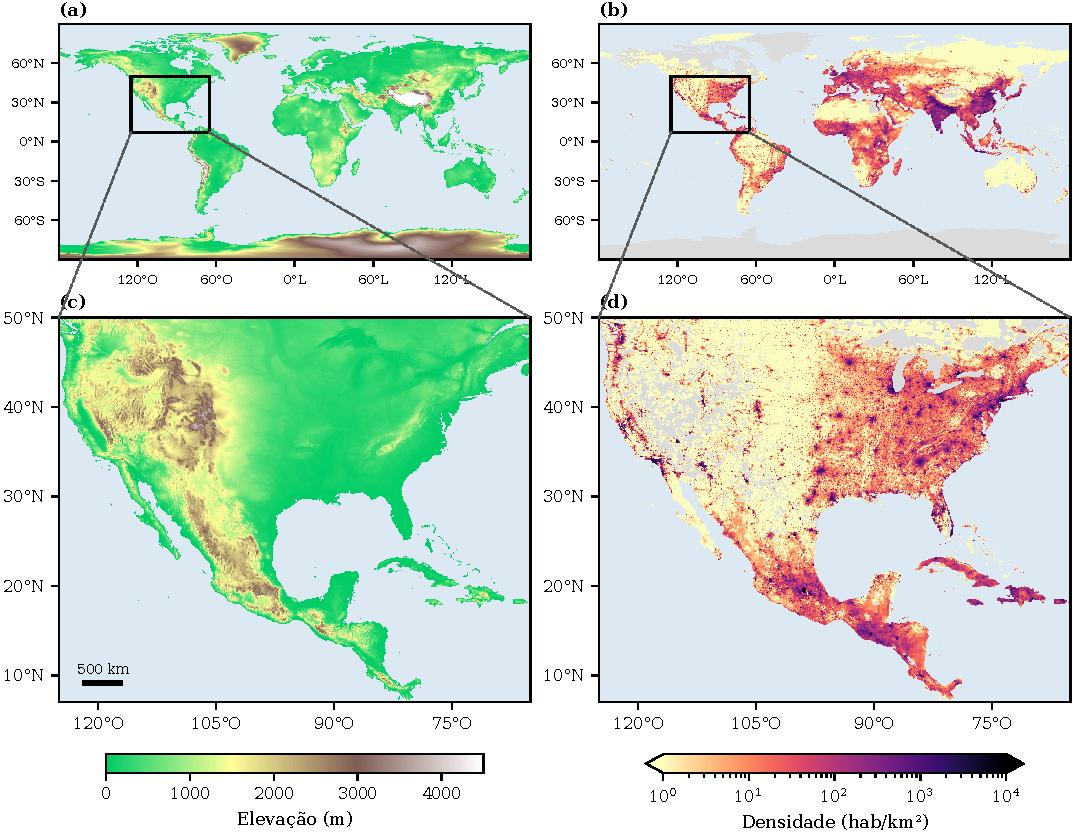
\includegraphics[width=\textwidth]{recorte}%
	}{%
		\Fonte{elaborado pelo autor a partir de \citeonline{gebco2024} e \citeonline{gpw4}.}%
		\Nota{(a) e (b): mundo, com o GEBCO lido de uma versão reduzida e o GPW somado em blocos de $40 \times 40$ células. (c) e (d): região de estudo. No painel (c) o oceano está em azul-claro; no painel (d), as células sem população estão em cinza.}%
	}
\end{figure}

\begin{figure}[ht!]
	\centering
	\Caption{\label{fig:pontos-coleta}Amostras do banco de microplásticos marinhos da NOAA no mundo e sítios do \textit{Nurdle Patrol} na região de estudo}
	\IBGEtab{}{%
		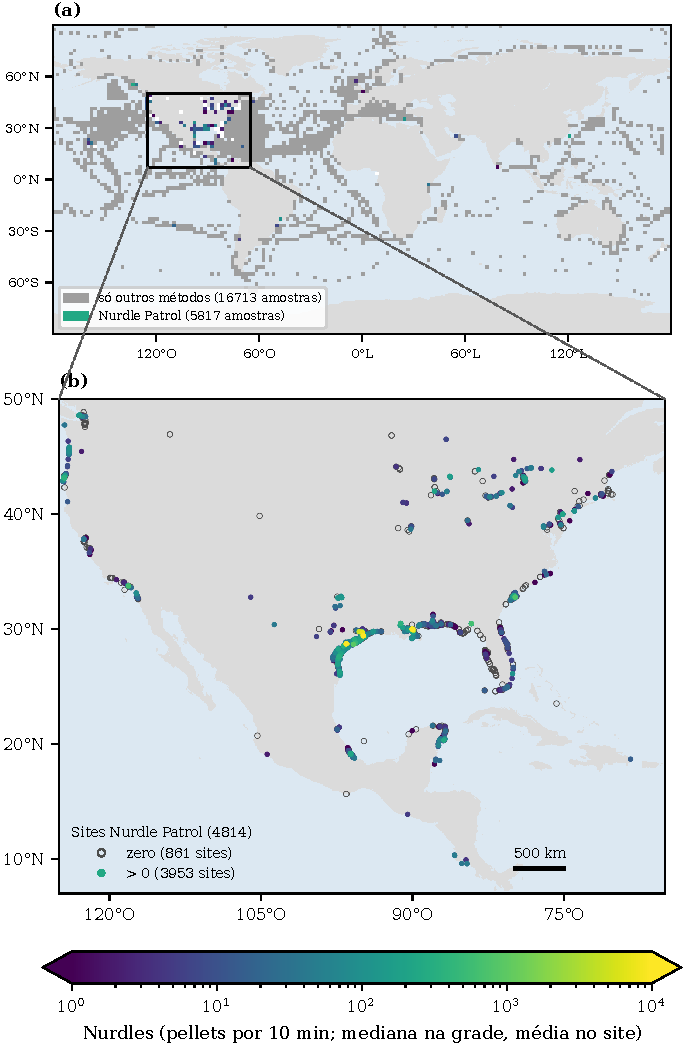
\includegraphics[width=0.78\textwidth]{pontos_coleta}%
	}{%
		\Fonte{elaborado pelo autor a partir de \citeonline{nyadjro2023}.}%
		\Nota{(a) Grade de $2^\circ$: em cor, a mediana das amostras do \textit{Nurdle Patrol} em cada célula; em cinza, células que só têm amostras de outros métodos. (b) Cada sítio do \textit{Nurdle Patrol} na região de estudo, com a média das suas amostras; círculos vazios indicam contagem zero.}%
	}
\end{figure}

\section{Bacias hidrográficas}
\label{sec:met-bacias}

\subsection{Resolução do relevo}

O IPBA disponível \cite{ipba} é implementado em Python puro: cada célula da grade é um objeto e os rótulos das bacias são gravados como inteiros sem sinal de 16 bits, o que limita o número de \textit{sinks} a 65.535. Com a resolução nativa do GEBCO, a região de estudo teria cerca de 150 milhões de células e centenas de milhares de \textit{sinks} costeiros. Por isso o relevo é reamostrado pela média em blocos de $8 \times 8$ células, passando para 2 minutos de arco ($\approx 3{,}7$ km). A grade resultante tem $1290 \times 1800 = 2{,}32$ milhões de células. A perda de resolução afeta sobretudo as bacias costeiras muito pequenas, que não entram na análise, e a posição exata das fozes, que passa a ser conhecida com precisão de um pixel.

\subsection{Oceano e \textit{sinks}}

O oceano é definido como o conjunto de células com altitude menor ou igual a zero \textbf{conectadas à borda da caixa}. A condição de conexão é importante: depressões interiores abaixo do nível do mar, como o Salton Sea e o Vale da Morte, na Califórnia, e o fundo dos Grandes Lagos, continuam sendo terra, porque não são fozes. Na região de estudo, 7.643 células abaixo de zero ficam no interior e são mantidas como terra.

Todo pixel de terra 4-vizinho de um pixel de oceano é declarado um \textit{sink}, com um rótulo próprio. O resultado são 11.851 \textit{sinks}, abaixo do limite de 65.535 do IPBA. Essa regra dispensa qualquer lista de rios ou de fozes: a bacia de um rio grande emerge sozinha, porque todas as células a montante escoam até o \textit{sink} da foz, enquanto os \textit{sinks} da costa entre duas fozes recebem apenas micro-bacias de encosta. O oceano entra no IPBA como ausência de dado, para que a percolação não atravesse o mar de uma bacia para outra.

\subsection{Delineamento e bacias principais}

O IPBA (\autoref{alg:ipba}) é executado sobre o relevo reamostrado com os \textit{sinks} costeiros e vizinhança de 4 células, sem condições de contorno periódicas. Cada célula de terra recebe o rótulo do \textit{sink} para o qual escoa, e cada \textit{sink} define uma bacia.

Como cada pixel de costa é um \textit{sink}, a maioria das bacias são micro-bacias de praia com poucas células. Para ficar apenas com as bacias de rio, as bacias são ordenadas por área, da maior para a menor, e são mantidas as de maior área até que a soma das áreas atinja uma fração $P$ da área de terra total; a bacia que cruza o limiar também é incluída. Com $P = 0{,}90$, esse critério seleciona as bacias principais sem nenhum limiar de área mínima. A área de cada célula é calculada em km$^2$ a partir das suas dimensões em graus, com o fator $\cos(\text{latitude})$ para a largura.

As bacias principais que tocam a borda da caixa ou o corte do Canal do Panamá são marcadas como \textbf{truncadas}, porque parte da sua área e da sua população pode estar fora do recorte. Elas não são excluídas da análise, mas são identificadas nos resultados.

\section{Manchas urbanas}
\label{sec:met-cca}

\subsection{Aplicação do CCA à grade do GPW}

Cada célula do GPW é um sítio do CCA localizado no seu centro. A densidade de cada célula é a sua população dividida pela sua área em km$^2$, calculada como na seção anterior. Uma célula é ativa se a sua densidade for maior que $D^{*}$, e duas células ativas estão ligadas se a distância entre os seus centros, calculada pela fórmula do haversine sobre uma esfera de raio 6.378,137 km, for menor que $\ell$. A implementação usada é a função \texttt{cca\_grid} do pacote CCA do grupo de pesquisa, que busca os vizinhos com uma árvore k-d sobre a esfera.

\subsection{Calibração de $D^{*}$ e $\ell$ pela lei de Zipf}
\label{sec:calibracao}

Os valores de $D^{*}$ e $\ell$ determinam quais regiões contam como cidades, e valores tomados de outros contextos não servem para esta região. Os valores usados numa versão anterior deste trabalho, calibrados para o semiárido brasileiro (30 hab/km$^2$ e 2 km), tornavam 98\% da população americana ``urbana''. O limiar de área urbana do censo americano, 1.000 hab/milha$^2$ ($\approx 386$ hab/km$^2$) \cite{census2020}, foi definido para os Estados Unidos e não necessariamente vale para o México e a América Central.

Por isso os dois parâmetros são escolhidos pela lei de Zipf, uma propriedade das cidades conhecida e independente do plástico. O procedimento tem quatro partes.

\textbf{Grade de parâmetros.} $D^{*}$ varia de 10 a 3.000 hab/km$^2$ em passos de 10, e $\ell$ varia de 100 a 5.000 m em passos de 100, num total de $300 \times 50 = 15.000$ combinações. Em cada combinação, calcula-se o expoente de Zipf das manchas resultantes.

\textbf{Varredura por união e busca.} Executar o CCA 15 mil vezes sobre uma grade de 37 milhões de células seria proibitivo. A varredura explora uma propriedade de monotonicidade: para um $\ell$ fixo, o conjunto de células ativas com limiar $D^{*}_1$ contém o conjunto ativo com qualquer limiar $D^{*}_2 > D^{*}_1$. Assim, se as células forem ativadas em ordem \textbf{decrescente} de densidade e cada célula nova for unida aos vizinhos já ativos a menos de $\ell$, as manchas presentes no momento em que a densidade cruza um valor $D^{*}$ da grade são exatamente as manchas do CCA com esse $D^{*}$. As uniões são feitas com uma estrutura de conjuntos disjuntos (\textit{union-find}) com união por tamanho e compressão de caminho \cite{tarjan1975}, a mesma ideia usada para rotular aglomerados em percolação \cite{hoshen1976,newmanziff2000}. O \autoref{alg:varredura} descreve o procedimento para um $\ell$.

\begin{algorithm}[ht!]
	\SetSpacedAlgorithm
	\caption{\label{alg:varredura}Varredura do CCA em $D^{*}$ para um $\ell$ fixo}
	\Entrada{densidades $\rho_k$ e populações $x_k$ das células; valores $D^{*}_1 > D^{*}_2 > \dots > D^{*}_m$; deslocamentos de vizinhança $\mathcal{V}_\ell$ válidos em cada linha da grade}
	\Saida{populações das manchas para cada $D^{*}_j$}
	\Inicio{
		ordena as células com $\rho_k > D^{*}_m$ em ordem decrescente de $\rho_k$\;
		$\mathit{pos} \leftarrow 1$\;
		\Para{$j \leftarrow 1$ \textbf{até} $m$}{
			\Enqto{$\rho_{k_{\mathit{pos}}} > D^{*}_j$}{
				$k \leftarrow k_{\mathit{pos}}$; \quad ativa $k$ como um conjunto unitário de população $x_k$\;
				\ParaCada{deslocamento $(\delta_i, \delta_j) \in \mathcal{V}_\ell$ válido na linha de $k$}{
					$q \leftarrow k + (\delta_i, \delta_j)$\;
					\Se{$q$ está ativa e $\mathrm{raiz}(q) \neq \mathrm{raiz}(k)$}{une os dois conjuntos, somando as populações\;}
				}
				$\mathit{pos} \leftarrow \mathit{pos} + 1$\;
			}
			registra as populações das raízes: são as manchas do CCA com $D^{*}_j$\;
		}
	}
\end{algorithm}

Os deslocamentos $\mathcal{V}_\ell$ são os pares $(\delta_i, \delta_j)$ de linhas e colunas cuja distância haversine é menor que $\ell$. Como a largura de uma célula em km diminui com a latitude, a validade de cada deslocamento é pré-calculada para cada linha da grade. Com isso, cada $\ell$ exige uma única passagem pelas células, e toda a coluna de 300 valores de $D^{*}$ sai dessa passagem. Valores de $\ell$ que não mudam o conjunto de deslocamentos válidos, por exemplo os menores que o espaçamento entre células, repetem o resultado anterior sem nova passagem. O algoritmo foi implementado com compilação just-in-time pelo Numba \cite{lam2015}, e a varredura completa leva cerca de 2 minutos e meio. A equivalência com o CCA foi verificada de duas formas: num raster de teste, a varredura reproduziu o \texttt{cca\_grid} em 600 combinações de parâmetros; e na região de estudo, o número de manchas e a população da maior mancha coincidem nos parâmetros escolhidos.

\textbf{Estimador do expoente.} Em cada combinação, o expoente de Zipf é estimado pelo estimador de Hill (\autoref{eq:hill}) sobre as $N$ maiores manchas, com $N = 50$, 100 e 200. Uma primeira versão usava o método CSN completo em cada combinação, com $x_{\min}$ escolhido pela distância KS, mas o $x_{\min}$ saltava de forma descontínua entre combinações vizinhas e o critério acabava escolhendo combinações degeneradas. O estimador de Hill com $N$ fixo é estável e mede exatamente o que a lei de Zipf descreve: a inclinação do topo do \textit{ranking}.

\textbf{Critério de escolha.} Os pares com $\alpha = 1$ formam uma curva no plano $(D^{*}, \ell)$, e não um ponto; é preciso um critério para escolher um par sobre ela. O critério adotado tem duas partes:

\begin{enumerate}
	\item \textbf{Piso físico para $\ell$.} São admitidos apenas valores $\ell \geq \ell_{\min} = 1.400$ m. A distância entre os centros de duas células do GPW vizinhas na diagonal chega a 1.307 m perto do equador. Com $\ell$ menor que isso, células vizinhas na diagonal não se ligam, e as manchas se fragmentam em faixas leste--oeste que não correspondem a cidades. Essas combinações podem produzir $\alpha \approx 1$ por acaso e precisam ser excluídas.
	\item \textbf{Zipf em vários tamanhos de amostra.} Entre as combinações admitidas, escolhe-se a que minimiza
	\begin{equation}
		\Delta(D^{*}, \ell) = \max_{N \in \{50,\,100,\,200\}} \left| \hat{\alpha}_N(D^{*}, \ell) - 1 \right|,
		\label{eq:delta}
	\end{equation}
	ou seja, a combinação em que o expoente fica mais próximo de 1 simultaneamente no topo do \textit{ranking} (50 maiores manchas) e mais abaixo nele (200 maiores).
\end{enumerate}

O par escolhido é verificado aplicando o \texttt{cca\_grid} com esses parâmetros e comparando as manchas com as da varredura. Como verificação independente, a distribuição completa das populações das manchas é ajustada pelo método CSN (\autoref{sec:estimacao}), com $x_{\min}$ escolhido pela distância KS, \textit{bootstrap} semiparamétrico com 200 réplicas para o valor-$p$ e comparação com as distribuições lognormal, exponencial e lei de potência truncada pela razão de Vuong.

A curva completa de pares com $\alpha_{100} \approx 1$ é exportada junto com o par escolhido, para que outros critérios possam ser comparados. Um princípio orientou todo o procedimento: os parâmetros do CCA \textbf{nunca} são ajustados para melhorar a correlação entre população e plástico, que só é calculada no segundo \textit{notebook}, depois de os parâmetros estarem fixados.

\subsection{Identificação das manchas}

Para inspeção dos resultados, as maiores manchas recebem o nome da cidade de referência mais próxima do seu centroide, calculado com a população como peso, a partir de uma lista de coordenadas de cerca de 30 metrópoles da região. O nome é usado apenas nas tabelas e figuras e não entra em nenhum cálculo.

\section{População por bacia}
\label{sec:met-populacao}

A população de uma bacia é a soma das populações das células do GPW dentro dela. Para fazer essa soma, o raster de bacias é levado para a grade do GPW pelo vizinho mais próximo, e não o contrário. A escolha da direção importa: o GPW é uma grade de \textbf{contagens}, e reamostrar contagens para uma grade mais grossa ou deslocada inventa ou duplica pessoas, enquanto o rótulo de bacia é uma variável categórica, que pode ser reamostrada sem perda de consistência.

Como a grade das bacias (2$'$) é mais grossa que a do GPW (30$''$), algumas células habitadas da linha de costa caem sobre um pixel que o relevo reamostrado classifica como oceano. Essas células são atribuídas à bacia de terra mais próxima, desde que ela esteja a no máximo 8 células do GPW ($\approx 7$ km). A população realocada e a que fica fora de qualquer bacia são reportadas nos resultados.

\textbf{Repartição das manchas urbanas.} Uma mancha urbana pode ficar sobre um divisor de águas, com parte da cidade drenando para uma bacia e parte para outra. Nesse caso a mancha é \textbf{dividida}: cada pedaço conta para a bacia em que está, porque é para lá que escoa a água, e com ela o lixo, que cai sobre ele. Uma versão anterior deste trabalho atribuía a mancha inteira à bacia que continha a maior parte da sua área, o que transferia populações inteiras para bacias vizinhas. A tabela de pedaços registra, para cada par (mancha, bacia), a população, a área e a fração da mancha naquela bacia. A população total de uma bacia não depende das manchas; elas servem para calcular a sua população urbana e para identificar quais cidades drenam para cada foz.

\section{Microplástico por bacia}
\label{sec:met-plastico}

\subsection{Sítios de coleta}

São usadas as amostras do \textit{Nurdle Patrol} com contagem definida dentro da caixa de estudo ampliada por uma margem de 50 km (o maior raio de aceitação testado), excluída a parte sul-americana. Amostras repetidas no mesmo par de coordenadas são agrupadas num \textbf{sítio}, cuja concentração é a média das contagens. O agrupamento evita que um ponto muito amostrado pese mais que os outros na associação com as bacias.

\subsection{O sítio mais próximo da foz}

A foz de cada bacia principal é o seu pixel-\textit{sink}, uma célula de $2' \times 2'$ na linha de costa. A distância entre a foz e cada sítio é calculada pelo haversine até o ponto do pixel mais próximo do sítio, e não até o centro do pixel: uma amostra coletada dentro do pixel da foz está a 0 km dela. Cada bacia principal recebe \textbf{o sítio mais próximo da sua foz} e dois valores de microplástico:

\begin{itemize}
	\item a \textbf{concentração}, em \textit{pellets} por 10 minutos, no sítio mais próximo;
	\item o \textbf{indicador de quantidade}, dado pela concentração multiplicada pela área da bacia (\textit{pellets}/10 min $\times$ km$^2$), que dá mais peso às bacias grandes, que drenam mais território.
\end{itemize}

Uma versão anterior deste trabalho atribuía a cada bacia a média de todas as amostras num círculo de 50 km ao redor da foz. Esse procedimento misturava fontes diferentes e fazia bacias vizinhas compartilharem as mesmas amostras, criando dependência artificial entre as observações. O sítio mais próximo, junto com a varredura do raio descrita a seguir, torna explícito o compromisso entre a proximidade da medição e o número de bacias.

\section{Raio de aceitação}
\label{sec:met-raio}

Uma bacia só tem microplástico ``medido'' se o seu sítio estiver perto da foz; um sítio a 100 km pode refletir outra bacia. Em vez de fixar um raio, o raio de aceitação $R$ é varrido de 1 a 50 km em passos de 1 km. Para cada $R$ são registrados:

\begin{itemize}
	\item a fração dos sítios que estão a até $R$ de alguma foz principal;
	\item o número de bacias com sítio a até $R$ e o número de sítios distintos entre elas, já que duas bacias vizinhas podem ter o mesmo sítio mais próximo;
	\item o expoente $\beta$, o seu IC de 95\% e o coeficiente $r$ das leis de escala da \autoref{sec:met-alometria}, para a concentração e para o indicador de quantidade.
\end{itemize}

Dois raios são destacados. O primeiro é $R = 1$ km, que corresponde a uma \textbf{medição garantida}: o sítio está no pixel da foz ou encostado nele. O segundo é $R_{\mathrm{maioria}}$, o \textbf{menor raio que contém a maioria} ($\geq 50\%$) dos sítios de coleta, que aproveita a maior parte da informação disponível sem aceitar distâncias arbitrariamente grandes.

\section{Alometria por bacia}
\label{sec:met-alometria}

Para cada raio, a lei de escala da \autoref{eq:escala} é ajustada entre a população $X$ da bacia e o microplástico $Y$ na foz, com cada bacia como uma observação. Os ajustes são feitos para as duas variáveis de resposta, concentração e indicador de quantidade, e seguem os passos abaixo.

\begin{enumerate}
	\item Entram as bacias com sítio a até $R$ da foz, população positiva e $Y > 0$. As contagens zero precisam sair do ajuste em escala log-log e são tratadas à parte, na discussão dos resultados.
	\item O expoente $\beta$ e o pré-fator $\log_{10} c$ são estimados por MQO sobre $\log_{10} X$ e $\log_{10} Y$.
	\item O IC de 95\% de $\beta$ e a banda de confiança da reta são obtidos por \textit{bootstrap} de pares com 10.000 reamostragens \cite{efron1979}.
	\item A significância é avaliada por um teste de permutação com 10.000 permutações dos valores de $Y$, com hipótese nula $\beta = 0$ \cite{good2005}.
	\item São reportados o coeficiente de Pearson $r$ entre os logaritmos e o coeficiente de Spearman $\rho_s$, com os respectivos valores-$p$.
	\item A influência de bacias individuais é avaliada por um teste \textit{leave-one-out}: o ajuste é refeito removendo uma bacia de cada vez, e registra-se a variação de $r$ e de $\beta$.
\end{enumerate}

O ajuste só é feito quando há pelo menos 5 bacias e 3 valores distintos de $Y$; abaixo disso, o resultado é reportado como dados insuficientes. A mesma bacia não entra duas vezes, mas duas bacias podem compartilhar o mesmo sítio; o número de sítios distintos é reportado junto com cada ajuste.

\section{Verificações das distribuições}
\label{sec:met-verificacoes}

Como verificação da consistência do \textit{pipeline}, três distribuições são ajustadas pelo método CSN com o pacote \texttt{powerlaw} \cite{alstott2014}: a área de todas as bacias delineadas que não tocam a borda, a população de todas as bacias e a população de todas as manchas urbanas. Redes fluviais têm distribuições de área em lei de potência com expoente $\gamma$ próximo de 1,4 a 1,5 para bacias aninhadas \cite{rodrigueziturbe1997,maritan1996}, e as manchas urbanas devem seguir aproximadamente a lei de Zipf ($\gamma \approx 2$). Em cada caso, a lei de potência é comparada com a lognormal e com a exponencial pela razão de Vuong.

\section{Implementação}
\label{sec:implementacao}

Todo o processamento foi implementado em Python, com NumPy \cite{harris2020}, SciPy \cite{virtanen2020}, pandas, xarray/rioxarray e rasterio para os dados em grade, Numba \cite{lam2015} para a varredura do CCA, \texttt{powerlaw} \cite{alstott2014} para os ajustes de cauda e Matplotlib \cite{hunter2007} para as figuras. O IPBA \cite{ipba} e o pacote CCA são clonados dos seus repositórios em tempo de execução. Os \textit{notebooks} foram desenvolvidos para o Google Colab, e todos os dados são baixados automaticamente. O \autoref{apendice:reprodutibilidade} lista os arquivos, os parâmetros e as saídas de cada etapa.

	\chapter{Resultados e discussão}
\label{chap:resultados}

Este capítulo apresenta os resultados na ordem do \textit{pipeline}: as bacias hidrográficas (\autoref{sec:res-bacias}), a calibração do CCA e as manchas urbanas (\autoref{sec:res-cca}), a repartição das manchas entre as bacias (\autoref{sec:res-reparticao}), o microplástico associado às fozes e o efeito do raio de aceitação (\autoref{sec:res-plastico}), as leis de escala entre população e microplástico (\autoref{sec:res-alometria}) e as verificações das distribuições (\autoref{sec:res-distribuicoes}). A \autoref{sec:discussao} discute o conjunto dos resultados e as suas limitações.

\section{Bacias hidrográficas}
\label{sec:res-bacias}

O relevo reamostrado tem 11.851 \textit{sinks} costeiros, e o IPBA produziu o mesmo número de bacias, uma por \textit{sink}. Ordenadas por área, as 138 maiores cobrem 90,0\% da área de terra da região de estudo (\autoref{fig:bacias}); as outras 11.713 são, na grande maioria, micro-bacias de encosta com poucas células. As bacias principais têm área mediana de 13.572 km$^2$, e a menor delas tem 4.897 km$^2$. Seis bacias principais tocam a borda da caixa ou o corte do Canal do Panamá e estão marcadas como truncadas; entre elas estão as duas maiores, a do Mississippi e a do São Lourenço, cujas cabeceiras mais ao norte ficam acima de 50$^\circ$N.

\begin{figure}[ht!]
	\centering
	\Caption{\label{fig:bacias}As 138 bacias principais, que cobrem 90\% da área de terra da região de estudo}
	\IBGEtab{}{%
		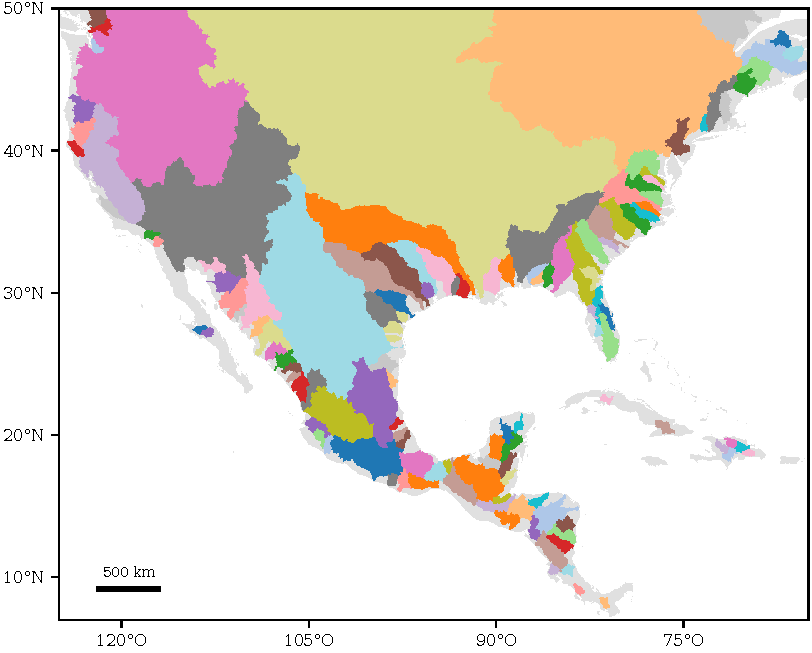
\includegraphics[width=\textwidth]{bacias_principais}%
	}{%
		\Fonte{elaborado pelo autor.}%
		\Nota{Cada bacia principal tem uma cor (as cores se repetem); as bacias costeiras menores estão em cinza-claro.}%
	}
\end{figure}

As bacias delineadas reproduzem as grandes bacias conhecidas do continente sem nenhuma informação além do relevo e da linha de costa. A bacia do Mississippi--Missouri ocupa o centro dos Estados Unidos, do oeste de Montana aos Apalaches; a do São Lourenço inclui os Grandes Lagos; a do Colorado drena o sudoeste até o Golfo da Califórnia; e a do Columbia drena o noroeste. No México aparecem as bacias do Rio Bravo (Rio Grande), do Pánuco, do Lerma--Santiago e do Balsas. A \autoref{tab:bacias-pop} lista as dez bacias principais mais populosas. Os nomes foram atribuídos a partir da coordenada da foz e não entram em nenhum cálculo.

\begin{table}[ht!]
	\centering
	\Caption{\label{tab:bacias-pop}As dez bacias principais mais populosas}
	\IBGEtab{}{%
		\small
		\begin{tabular}{llrrrr}
			\toprule
			\textbf{Bacia} & \textbf{Foz (lon, lat)} & \textbf{Área (km$^2$)} & \textbf{População (mi)} & \textbf{\% urbana} & \textbf{Sítio (km)} \\
			\midrule
			Mississippi--Atchafalaya$^{*}$ & $-91{,}18$; $29{,}58$ & 3.150.557 & 70,20 & 45 & 37,8 \\
			São Lourenço$^{*}$ & $-70{,}88$; $46{,}92$ & 1.374.739 & 61,10 & 60 & 316,9 \\
			Pánuco & $-97{,}85$; $22{,}35$ & 166.272 & 31,50 & 84 & 114,5 \\
			Rio Bravo (Rio Grande) & $-97{,}32$; $26{,}28$ & 849.584 & 24,24 & 84 & 9,7 \\
			Lerma--Santiago & $-105{,}38$; $21{,}58$ & 133.470 & 22,60 & 75 & 92,3 \\
			Balsas & $-102{,}18$; $17{,}95$ & 117.024 & 16,55 & 65 & 260,9 \\
			Colorado & $-114{,}82$; $31{,}85$ & 809.665 & 15,87 & 73 & 229,9 \\
			Columbia$^{*}$ & $-123{,}58$; $46{,}22$ & 1.012.275 & 12,86 & 64 & 35,7 \\
			Sacramento--San Joaquin & $-122{,}25$; $38{,}08$ & 177.542 & 9,85 & 75 & 21,3 \\
			Mobile & $-87{,}98$; $30{,}72$ & 171.579 & 8,62 & 18 & 2,0 \\
			\bottomrule
		\end{tabular}%
	}{%
		\Fonte{elaborado pelo autor.}%
		\Nota{$^{*}$ bacia truncada pela borda da caixa. ``\% urbana'' é a fração da população da bacia que vive em manchas urbanas do CCA. ``Sítio'' é a distância da foz ao sítio do \textit{Nurdle Patrol} mais próximo.}%
	}
\end{table}

A população somada das 138 bacias principais é de 450,4 milhões de habitantes, 74\% dos 606,6 milhões da região de estudo; o restante vive nas bacias costeiras menores, que concentram cidades litorâneas como Nova York e boa parte da Flórida. Na passagem das bacias para a grade do GPW, 8,5 milhões de habitantes de células da linha de costa foram realocados para a bacia de terra mais próxima, e apenas 168.498 habitantes ficaram fora de qualquer bacia.

\section{Calibração do CCA e manchas urbanas}
\label{sec:res-cca}

\subsection{Matriz de expoentes}

A \autoref{fig:zipf-matriz} mostra o expoente $\hat{\alpha}_{100}$ nas 15.000 combinações de $(D^{*}, \ell)$ e o desvio $\Delta$ da \autoref{eq:delta}. Abaixo de cerca de 1.000 m, $\ell$ é menor que o espaçamento entre células na mesma coluna ($\approx 927$ m), e só se ligam células vizinhas na mesma linha em latitudes altas, onde as células são mais estreitas; quase toda célula ativa é uma mancha, e o expoente fica entre 0,3 e 0,6, refletindo sobretudo a distribuição das densidades das células. Entre 1.000 e 1.300 m, as células se ligam na horizontal e na vertical, mas perto do equador ainda não na diagonal, e aparecem as manchas degeneradas descritas na \autoref{sec:calibracao}. A partir de $\ell_{\min} = 1.400$ m, a curva $\hat{\alpha}_{100} = 1$ atravessa a matriz em valores de $D^{*}$ entre cerca de 400 e 1.100 hab/km$^2$.

\begin{figure}[ht!]
	\centering
	\Caption{\label{fig:zipf-matriz}Expoente de Zipf e desvio $\Delta$ na grade de parâmetros do CCA}
	\IBGEtab{}{%
		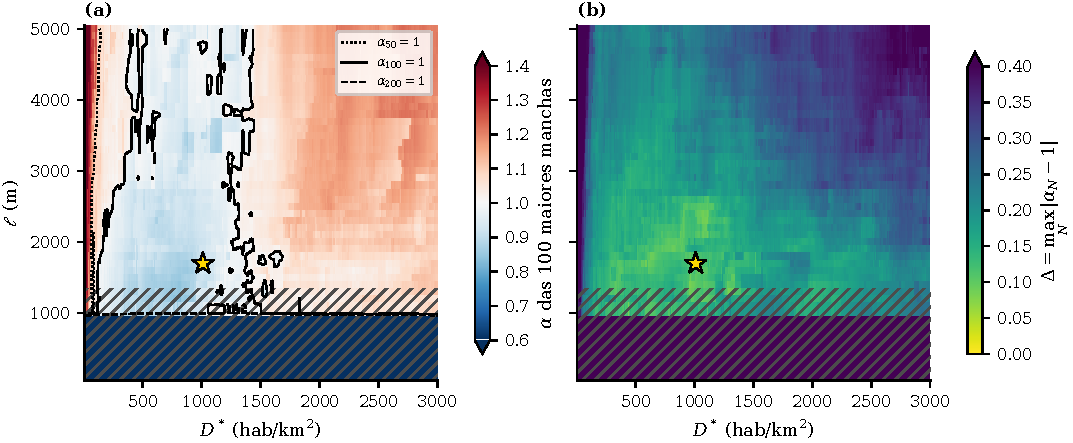
\includegraphics[width=\textwidth]{zipf_matriz}%
	}{%
		\Fonte{elaborado pelo autor.}%
		\Nota{(a) $\hat{\alpha}_{100}$ em cada combinação de $D^{*}$ e $\ell$, com as curvas $\hat{\alpha}_N = 1$ para $N = 50$, 100 e 200. (b) Desvio $\Delta = \max_N |\hat{\alpha}_N - 1|$. A faixa hachurada, $\ell < \ell_{\min} = 1.400$ m, é excluída da escolha; a estrela marca o par escolhido.}%
	}
\end{figure}

A \autoref{tab:calibracao} mostra, para cada $\ell$ entre 1.400 e 2.600 m, o $D^{*}$ que minimiza $\Delta$. O mínimo global ocorre em $\ell = 1.700$ m e $D^{*} = 1.010$ hab/km$^2$, com $\Delta = 0{,}081$. O mínimo é raso: todos os valores de $\ell$ entre 1.400 e 2.400 m têm um $D^{*}$ com $\Delta < 0{,}10$, e o $D^{*}$ ótimo fica entre 820 e 1.110 hab/km$^2$ em quase todos eles. Em todas as linhas da tabela, $\hat{\alpha}_{200}$ é maior que 1 e é ele que determina $\Delta$; os expoentes do topo, $\hat{\alpha}_{50}$ e $\hat{\alpha}_{100}$, ficam entre 0,90 e 0,97. Esse padrão, em que o expoente cresce com $N$, é discutido na \autoref{sec:res-rank-size}.

\begin{table}[ht!]
	\centering
	\Caption{\label{tab:calibracao}Melhor $D^{*}$ para cada $\ell$ admitido pelo critério $\Delta$}
	\IBGEtab{}{%
		\small
		\begin{tabular}{rrrrrr}
			\toprule
			\textbf{$\ell$ (m)} & \textbf{$D^{*}$ (hab/km$^2$)} & \textbf{$\Delta$} & \textbf{$\hat{\alpha}_{50}$} & \textbf{$\hat{\alpha}_{100}$} & \textbf{$\hat{\alpha}_{200}$} \\
			\midrule
			1.400 & 960 & 0,081 & 0,919 & 0,926 & 1,053 \\
			1.500 & 970 & 0,088 & 0,917 & 0,912 & 1,079 \\
			1.600 & 1.040 & 0,098 & 0,903 & 0,917 & 1,098 \\
			\textbf{1.700} & \textbf{1.010} & \textbf{0,081} & \textbf{0,925} & \textbf{0,939} & \textbf{1,081} \\
			1.800 & 630 & 0,090 & 0,910 & 0,915 & 1,088 \\
			1.900 & 820 & 0,091 & 0,959 & 0,909 & 1,089 \\
			2.000 & 850 & 0,097 & 0,942 & 0,903 & 1,096 \\
			2.100 & 1.110 & 0,090 & 0,936 & 0,945 & 1,090 \\
			2.200 & 1.100 & 0,093 & 0,963 & 0,950 & 1,093 \\
			2.300 & 1.110 & 0,083 & 0,965 & 0,942 & 1,083 \\
			2.400 & 1.110 & 0,085 & 0,952 & 0,947 & 1,085 \\
			2.500 & 1.110 & 0,100 & 0,962 & 0,959 & 1,100 \\
			2.600 & 1.110 & 0,108 & 0,961 & 0,965 & 1,108 \\
			\bottomrule
		\end{tabular}%
	}{%
		\Fonte{elaborado pelo autor.}%
		\Nota{Em negrito, o par escolhido. Para $\ell > 2.600$ m, o menor $\Delta$ passa de 0,13.}%
	}
\end{table}

O par escolhido tem uma interpretação física razoável. O limiar de 1.010 hab/km$^2$ é cerca de 2,6 vezes o limiar de área urbana do censo americano (386 hab/km$^2$) \cite{census2020}, o que é esperado, já que o GPW distribui a população de cada unidade censitária de forma homogênea e suaviza os picos de densidade. A distância de 1,7 km é pouco maior que a diagonal entre células vizinhas, o que significa que as manchas são praticamente conjuntos de células ativas contíguas, com tolerância para vãos de uma célula.

\subsection{Manchas urbanas}

Com $D^{*} = 1.010$ hab/km$^2$ e $\ell = 1.700$ m, o CCA identifica 12.185 manchas urbanas, que somam 349,5 milhões de habitantes, 58\% da população da região. O \texttt{cca\_grid} aplicado com esses parâmetros produziu exatamente o mesmo número de manchas e a mesma população da maior mancha que a varredura (20.602.596 habitantes), confirmando a equivalência entre os dois procedimentos. A \autoref{tab:top-manchas} lista as dez maiores manchas. Sem nenhuma lista de cidades fornecida ao algoritmo, elas correspondem às grandes metrópoles da região, com os centroides a poucos quilômetros dos centros urbanos.

\begin{table}[ht!]
	\centering
	\Caption{\label{tab:top-manchas}As dez maiores manchas urbanas ($D^{*} = 1.010$ hab/km$^2$, $\ell = 1.700$ m)}
	\IBGEtab{}{%
		\small
		\begin{tabular}{rlrrrr}
			\toprule
			\textbf{Posto} & \textbf{Mancha} & \textbf{População} & \textbf{Área (km$^2$)} & \textbf{Densidade (hab/km$^2$)} & \textbf{Centroide (lon, lat)} \\
			\midrule
			1 & Cidade do México & 20.602.596 & 2.204 & 9.349 & $-99{,}10$; $19{,}45$ \\
			2 & Nova York & 15.482.384 & 3.316 & 4.669 & $-73{,}92$; $40{,}75$ \\
			3 & Los Angeles & 14.240.127 & 4.017 & 3.545 & $-118{,}03$; $33{,}98$ \\
			4 & Chicago & 6.335.092 & 2.253 & 2.812 & $-87{,}83$; $41{,}85$ \\
			5 & Toronto & 6.029.628 & 1.372 & 4.394 & $-79{,}49$; $43{,}71$ \\
			6 & Miami & 5.329.254 & 2.073 & 2.570 & $-80{,}24$; $26{,}05$ \\
			7 & Guadalajara & 5.073.091 & 594 & 8.547 & $-103{,}35$; $20{,}63$ \\
			8 & Monterrey & 4.971.276 & 637 & 7.800 & $-100{,}28$; $25{,}72$ \\
			9 & Houston & 4.814.175 & 1.982 & 2.429 & $-95{,}46$; $29{,}76$ \\
			10 & Santo Domingo & 4.737.554 & 947 & 5.004 & $-69{,}92$; $18{,}50$ \\
			\bottomrule
		\end{tabular}%
	}{%
		\Fonte{elaborado pelo autor a partir de \citeonline{gpw4}.}%
	}
\end{table}

A tabela tem duas particularidades. A primeira é que as manchas mexicanas e caribenhas são mais densas que as americanas: Cidade do México, Guadalajara e Monterrey têm mais de 7.800 hab/km$^2$, contra 2.400 a 4.700 hab/km$^2$ nas metrópoles dos Estados Unidos, o que reflete a forma mais compacta dessas cidades. A segunda é um artefato do GPW em Monterrey: cerca de 3 milhões de pessoas estão concentradas em uns 20 pixels, com densidades de até 810 mil hab/km$^2$, fisicamente impossíveis. O artefato provavelmente vem de uma unidade censitária muito pequena que recebeu uma população grande. Ele não muda a mancha, porque todas essas células já estão acima de $D^{*}$ e a população total é a mesma, mas mostra que valores de densidade de células individuais do GPW precisam ser lidos com cautela. O dado não foi alterado.

\subsection{Distribuição \textit{rank-size}}
\label{sec:res-rank-size}

A \autoref{fig:zipf} mostra a distribuição \textit{rank-size} das manchas. No topo do \textit{ranking}, a distribuição segue de perto a lei de Zipf: os estimadores de Hill dão $\hat{\alpha}_{50} = 0{,}925$, $\hat{\alpha}_{100} = 0{,}939$ e $\hat{\alpha}_{200} = 1{,}081$. Mais abaixo no \textit{ranking}, a curva fica mais íngreme. O ajuste CSN sobre a cauda escolhe $x_{\min} = 21.121$ habitantes, com 1.325 manchas na cauda, e dá $\hat{\gamma} = 1{,}822 \pm 0{,}023$, ou seja, $\hat{\alpha} = 1{,}217 \pm 0{,}033$. A distância KS é 0,017, abaixo do valor crítico de 0,037, e o \textit{bootstrap} dá $p = 0{,}08$, próximo do limiar convencional de 0,1. A regressão log-log sobre a mesma cauda dá $\alpha = 1{,}16$ ($R^2 = 0{,}994$).

\begin{figure}[ht!]
	\centering
	\Caption{\label{fig:zipf}Distribuição \textit{rank-size} das 12.185 manchas urbanas}
	\IBGEtab{}{%
		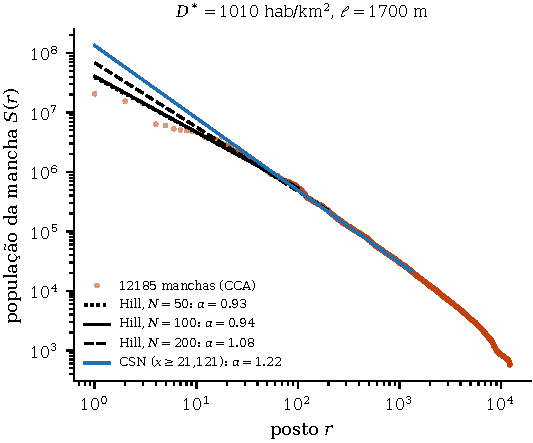
\includegraphics[width=0.85\textwidth]{zipf}%
	}{%
		\Fonte{elaborado pelo autor.}%
		\Nota{Retas de Hill para as 50, 100 e 200 maiores manchas e reta do ajuste CSN sobre a cauda ($x \geq x_{\min}$).}%
	}
\end{figure}

A distribuição é, portanto, \textbf{côncava} no gráfico log-log: o expoente cresce à medida que se incluem manchas menores. A comparação pela razão de Vuong confirma essa leitura. A lei de potência é fortemente preferida à exponencial ($R = 8{,}64$, $p < 10^{-17}$), não se distingue da lognormal ($R = -1{,}29$, $p = 0{,}20$) e perde para a lei de potência truncada ($R = -2{,}52$, $p = 0{,}004$), que tem exatamente essa curvatura. O resultado concorda com a literatura: \citeonline{eeckhout2004} mostrou que a distribuição completa das cidades americanas é lognormal e que a lei de Zipf vale apenas na cauda superior, e \citeonline{rozenfeld2011} encontraram a lei de Zipf nas manchas do CCA acima de um tamanho mínimo. A conclusão prática é que a calibração garante a lei de Zipf para as maiores manchas, que são as que mais pesam na população das bacias, mas não para a distribuição inteira.

\section{Repartição das manchas entre as bacias}
\label{sec:res-reparticao}

Das 12.185 manchas, 618 cruzam divisores de água e foram divididas entre duas ou mais bacias. São poucas em número, mas grandes: somam 41\% da população urbana, o que mostra que a repartição não é um detalhe. A \autoref{fig:manchas-fozes} mostra as dez maiores manchas e as fozes das bacias principais que recebem pedaços delas, e a \autoref{fig:mapa-integrado} sobrepõe as bacias, as manchas e os sítios de coleta.

\begin{figure}[ht!]
	\centering
	\Caption{\label{fig:manchas-fozes}As dez maiores manchas urbanas e as fozes das bacias principais em que se dividem}
	\IBGEtab{}{%
		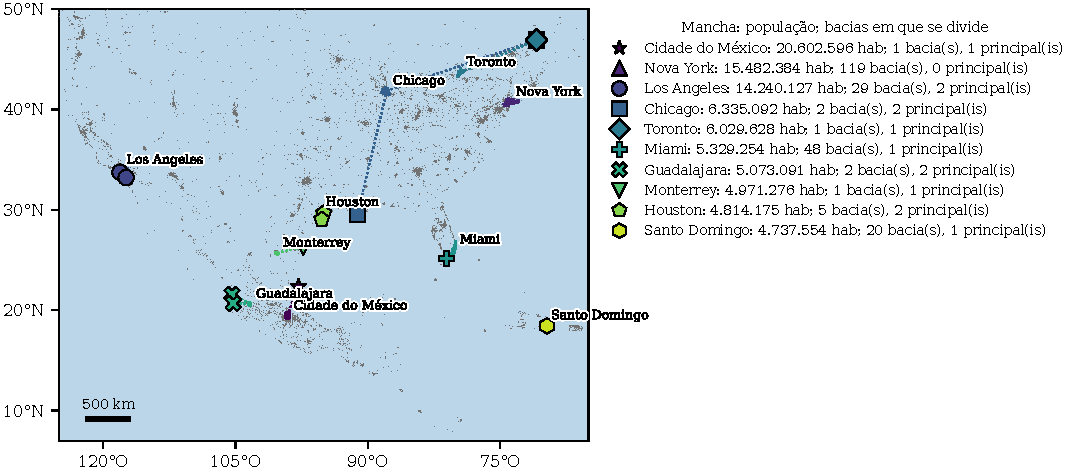
\includegraphics[width=\textwidth]{mapa_manchas_fozes}%
	}{%
		\Fonte{elaborado pelo autor.}%
		\Nota{Cada mancha tem uma cor e um símbolo; o símbolo marca a foz de cada bacia principal que recebe um pedaço da mancha, ligada ao centroide por uma linha pontilhada. Na exibição, as dez manchas foram dilatadas em cerca de 11 km para ficarem visíveis na escala continental. As demais manchas estão em cinza.}%
	}
\end{figure}

Os casos das maiores manchas ilustram os três comportamentos possíveis.

\begin{itemize}
	\item \textbf{Mancha inteira numa bacia principal.} A Cidade do México está 100\% na bacia do Pánuco, que deságua no Golfo do México perto de Tampico, a mais de 300 km da cidade; o mesmo vale para Guadalajara (Lerma--Santiago), Monterrey (Rio Bravo) e Toronto (São Lourenço). São casos em que o método atribui a população a uma foz distante, que uma análise baseada em proximidade costeira não encontraria.
	\item \textbf{Mancha dividida entre bacias principais.} Chicago fica sobre o divisor entre o Lago Michigan e o rio Illinois: 83\% da mancha drena para o São Lourenço e 17\% para o Mississippi. Houston se divide entre cinco bacias, duas delas principais.
	\item \textbf{Mancha em bacias costeiras pequenas.} Nova York se divide entre 119 bacias, nenhuma delas principal; o maior pedaço tem 10\% da mancha. Com um \textit{sink} por pixel de costa, a Baía de Nova York e a foz do Hudson se fragmentam em muitas micro-bacias na grade de 2$'$, e a cidade não é associada a nenhuma bacia de rio. Los Angeles e Miami têm comportamento semelhante: cerca de 40\% e 56\% das manchas, respectivamente, ficam em bacias principais, e o restante se espalha por dezenas de bacias costeiras.
\end{itemize}

\begin{figure}[ht!]
	\centering
	\Caption{\label{fig:mapa-integrado}Bacias principais, manchas urbanas, sítios de coleta e fozes}
	\IBGEtab{}{%
		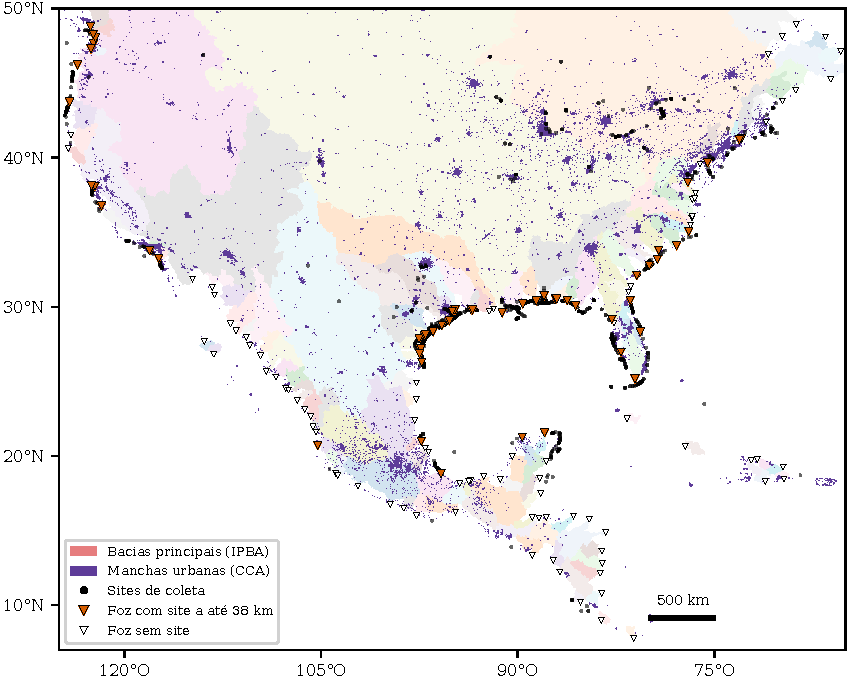
\includegraphics[width=\textwidth]{mapa_integrado}%
	}{%
		\Fonte{elaborado pelo autor.}%
		\Nota{Triângulos cheios: fozes com sítio do \textit{Nurdle Patrol} a até $R_{\mathrm{maioria}} = 38$ km; triângulos vazios: fozes sem sítio nesse raio.}%
	}
\end{figure}

O último caso é uma limitação importante. Grandes cidades litorâneas que ficam em estuários fragmentados, como Nova York, são justamente as que mais poderiam contribuir com plástico para o mar e ficam fora das bacias principais. Uma solução seria agrupar os \textit{sinks} de uma mesma baía ou estuário antes de rodar o IPBA, o que é discutido como trabalho futuro no \autoref{chap:conclusao}.

\section{Microplástico nas fozes e raio de aceitação}
\label{sec:res-plastico}

Dentro da caixa ampliada pela margem de 50 km há 5.783 amostras do \textit{Nurdle Patrol} em 4.814 sítios distintos, dos quais 861 têm contagem média zero. A distribuição espacial é muito desigual (\autoref{fig:pontos-coleta}): a maior parte dos sítios está na costa do Golfo do México, do Texas à Flórida, com grupos menores na costa atlântica, na costa do Pacífico e nos Grandes Lagos, e poucos sítios no México, na América Central e no Caribe. A distância mediana entre a foz de uma bacia principal e o sítio mais próximo é de 88,1 km, e apenas 6 das 138 fozes têm um sítio a até 1 km.

A \autoref{fig:varredura} e a \autoref{tab:varredura} mostram o efeito do raio de aceitação. A fração dos sítios a até $R$ de alguma foz principal cresce devagar até cerca de 30 km e acelera depois disso; o menor raio que contém a maioria dos sítios é $R_{\mathrm{maioria}} = 38$ km, com 53\% deles. O número de bacias com sítio e contagem positiva cresce rápido nos primeiros 10 km, chegando a 21, e depois devagar, até 33 em 50 km.

\begin{figure}[ht!]
	\centering
	\Caption{\label{fig:varredura}Efeito do raio de aceitação entre a foz e o sítio de coleta}
	\IBGEtab{}{%
		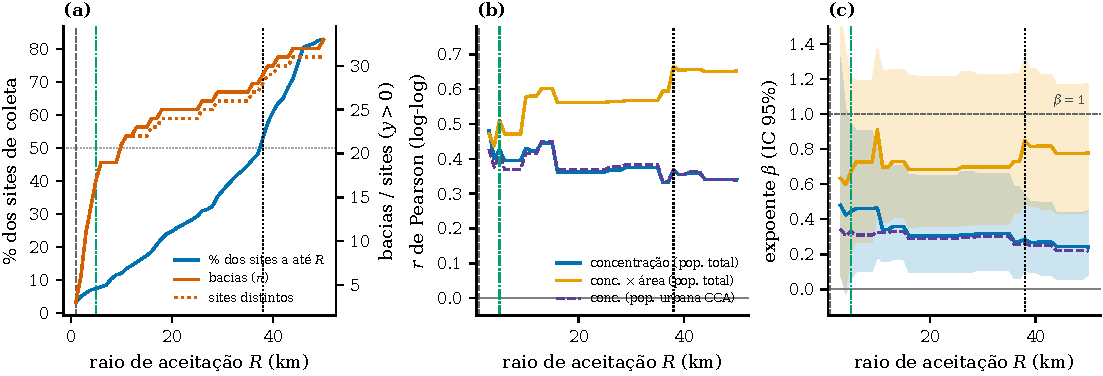
\includegraphics[width=\textwidth]{varredura_raio}%
	}{%
		\Fonte{elaborado pelo autor.}%
		\Nota{(a) Fração dos sítios a até $R$ de uma foz principal, número de bacias com sítio e número de sítios distintos. (b) Coeficiente de Pearson $r$ entre os logaritmos da população e do microplástico. (c) Expoente $\beta$ com IC de 95\%. Linha tracejada: $R = 1$ km; linha pontilhada: $R_{\mathrm{maioria}} = 38$ km. Só entram as bacias com contagem positiva.}%
	}
\end{figure}

\begin{table}[ht!]
	\centering
	\Caption{\label{tab:varredura}Leis de escala entre população e microplástico em função do raio de aceitação}
	\IBGEtab{}{%
		\small
		\begin{tabular}{rrrrrrrrr}
			\toprule
			& & & & \multicolumn{3}{c}{\textbf{Concentração}} & \multicolumn{2}{c}{\textbf{Conc. $\times$ área}} \\
			\cmidrule(lr){5-7} \cmidrule(lr){8-9}
			\textbf{$R$ (km)} & \textbf{\% sítios} & \textbf{Bacias} & \textbf{Sítios} & \textbf{$\beta$} & \textbf{$r$} & \textbf{$p$} & \textbf{$\beta$} & \textbf{$r$} \\
			\midrule
			1 & 3,3 & 3 & 3 & -- & -- & -- & -- & -- \\
			2 & 5,2 & 6 & 6 & 0,386 & 0,936 & 0,006 & 0,313 & 0,486 \\
			5 & 7,5 & 17 & 17 & 0,443 & 0,427 & 0,088 & 0,672 & 0,511 \\
			10 & 12,1 & 21 & 21 & 0,464 & 0,430 & 0,052 & 0,912 & 0,578 \\
			20 & 24,8 & 25 & 24 & 0,306 & 0,363 & 0,075 & 0,683 & 0,562 \\
			30 & 37,1 & 27 & 26 & 0,318 & 0,376 & 0,054 & 0,699 & 0,567 \\
			\textbf{38} & \textbf{53,0} & \textbf{29} & \textbf{28} & \textbf{0,283} & \textbf{0,367} & \textbf{0,050} & \textbf{0,849} & \textbf{0,665} \\
			40 & 61,0 & 30 & 29 & 0,267 & 0,355 & 0,054 & 0,816 & 0,655 \\
			50 & 82,8 & 33 & 31 & 0,243 & 0,339 & 0,054 & 0,778 & 0,652 \\
			\bottomrule
		\end{tabular}%
	}{%
		\Fonte{elaborado pelo autor.}%
		\Nota{``Bacias'': bacias principais com sítio a até $R$ e contagem positiva; ``Sítios'': sítios distintos entre elas. $p$ é o valor-$p$ do coeficiente de Pearson. Com $R = 1$ km há apenas 3 bacias com contagem positiva, insuficientes para o ajuste.}%
	}
\end{table}

\textbf{Medição garantida ($R = 1$ km).} Seis bacias principais têm um sítio a até 1 km da foz, mas três delas têm contagem zero, e restam apenas três com contagem positiva: as de Los Angeles (San Gabriel), a de Galveston--Houston e uma pequena bacia do sul do Texas. Com três pontos não é possível ajustar uma lei de escala nem avaliar a sua significância. O painel (a) da \autoref{fig:dispersao} mostra esses pontos apenas para referência.

\textbf{Raios pequenos.} Com $R = 2$ km, as seis bacias com contagem positiva dão $r = 0{,}94$ ($p = 0{,}006$) para a concentração. O valor é alto, mas se apoia em seis pontos e cai para cerca de 0,43 já em $R = 5$ km, com 17 bacias. Ele é um exemplo do risco de escolher o raio pelo resultado: a varredura mostra que valores altos de $r$ em raios pequenos são flutuações de amostras minúsculas.

\textbf{Estabilidade a partir de 10 km.} De 10 a 50 km, o $r$ da concentração fica entre 0,34 e 0,45 e o $\beta$ entre 0,24 e 0,47, com valores-$p$ entre 0,05 e 0,09. Para o indicador de quantidade, $r$ fica entre 0,56 e 0,67 e $\beta$ entre 0,68 e 0,91. A relação é, portanto, estável em relação ao raio, mas fraca e no limite da significância estatística convencional para a concentração.

\section{Leis de escala entre população e microplástico}
\label{sec:res-alometria}

A \autoref{fig:dispersao} mostra as relações entre a população das bacias e o microplástico nas fozes, e a \autoref{tab:escala} resume os ajustes para $R_{\mathrm{maioria}} = 38$ km. As 29 bacias com contagem positiva usam 28 sítios distintos.

\begin{figure}[ht!]
	\centering
	\Caption{\label{fig:dispersao}População das bacias versus microplástico na foz}
	\IBGEtab{}{%
		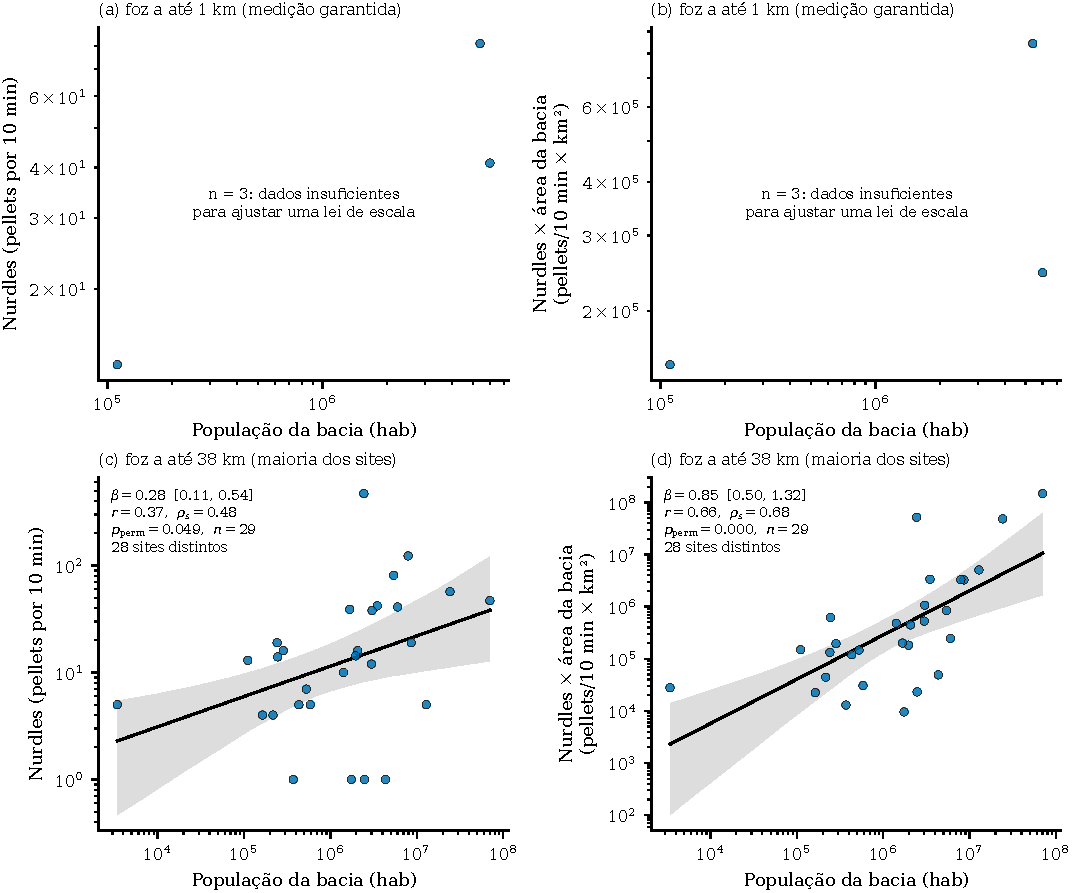
\includegraphics[width=\textwidth]{dispersao_pop_lixo}%
	}{%
		\Fonte{elaborado pelo autor.}%
		\Nota{(a) e (b): bacias com sítio a até 1 km da foz. (c) e (d): bacias com sítio a até $R_{\mathrm{maioria}} = 38$ km. Em (a) e (c), concentração de \textit{pellets}; em (b) e (d), concentração multiplicada pela área da bacia. Retas: MQO em log-log; faixas: banda de confiança de 95\% por \textit{bootstrap}.}%
	}
\end{figure}

\begin{table}[ht!]
	\centering
	\Caption{\label{tab:escala}Leis de escala entre população da bacia e microplástico na foz ($R = 38$ km)}
	\IBGEtab{}{%
		\small
		\begin{tabular}{lrrrrrrr}
			\toprule
			\textbf{Variável} & \textbf{$n$} & \textbf{$\beta$} & \textbf{IC 95\%} & \textbf{$p_{\mathrm{perm}}$} & \textbf{$r$} & \textbf{$\rho_s$} & \textbf{$R^2$} \\
			\midrule
			Concentração & 29 & 0,283 & [0,108; 0,539] & 0,049 & 0,367 & 0,480 & 0,135 \\
			Concentração $\times$ área & 29 & 0,849 & [0,503; 1,321] & $<0{,}001$ & 0,665 & 0,684 & 0,442 \\
			\bottomrule
		\end{tabular}%
	}{%
		\Fonte{elaborado pelo autor.}%
		\Nota{IC por \textit{bootstrap} de pares (10.000 reamostragens); $p_{\mathrm{perm}}$ por permutação (10.000 permutações).}%
	}
\end{table}

\textbf{Concentração.} A concentração de \textit{pellets} na foz cresce com a população da bacia segundo um expoente $\beta = 0{,}28$, com IC de 95\% de 0,11 a 0,54, que exclui o zero, e $p_{\mathrm{perm}} = 0{,}049$. A relação é fortemente \textbf{sublinear}: dobrar a população da bacia está associado a um aumento de apenas $2^{0{,}28} - 1 \approx 21\%$ na concentração. A dispersão é grande: $r = 0{,}37$ e $R^2 = 0{,}13$, ou seja, a população explica cerca de 13\% da variância do logaritmo da concentração. A correlação de postos é um pouco maior, $\rho_s = 0{,}48$ ($p = 0{,}008$), o que indica que parte da fraqueza do ajuste linear vem de pontos extremos, como a bacia com 471 \textit{pellets} por 10 minutos na costa central do Texas.

\textbf{Indicador de quantidade.} Multiplicando a concentração pela área da bacia, o expoente sobe para $\beta = 0{,}85$ (IC de 0,50 a 1,32), com $r = 0{,}66$ e $p_{\mathrm{perm}} < 0{,}001$. O resultado parece muito mais forte, mas a maior parte dele vem da área, e não do plástico. Como $\log(\text{concentração} \times A) = \log(\text{concentração}) + \log A$, e o MQO é linear, o expoente do indicador de quantidade é a soma do expoente da concentração com o expoente da área em função da população: $0{,}85 = 0{,}28 + 0{,}57$. Nas bacias com sítio, a área e a população estão fortemente correlacionadas ($\rho_s = 0{,}67$, $p < 10^{-7}$), porque bacias maiores tendem a ter mais gente. O indicador de quantidade herda essa correlação, que existiria mesmo que a concentração de plástico fosse aleatória. Ele não deve, portanto, ser lido como evidência independente de que a população determina o plástico.

\textbf{Contagens zero.} Das 52 bacias principais com sítio a até 38 km, 23 têm contagem zero e ficam fora dos ajustes em log-log. A exclusão não é neutra: se as bacias com zero fossem sistematicamente menos populosas, excluí-las aumentaria artificialmente a inclinação. Os dados não indicam esse viés: a população mediana das bacias com zero é de 1,10 milhão de habitantes, contra 1,97 milhão nas bacias com contagem positiva, diferença que não é significativa (teste de Mann--Whitney, $p = 0{,}50$). Mas a inclusão dos zeros enfraquece a associação. Com as 52 bacias, a correlação de postos entre população e concentração cai para $\rho_s = 0{,}25$ ($p = 0{,}07$), e entre população e indicador de quantidade para $\rho_s = 0{,}32$ ($p = 0{,}02$).

\textbf{Influência de bacias individuais.} O teste \textit{leave-one-out} (\autoref{fig:loo}) mostra que nenhuma bacia isolada determina o resultado da concentração: removendo uma bacia de cada vez, $r$ varia de 0,33 a 0,43 e $\beta$ de 0,25 a 0,35. As bacias de maior influência são as mais populosas, Mississippi e Rio Bravo, cuja remoção reduz $r$ em cerca de 0,035, e uma bacia do noroeste da Flórida, com foz perto de Panama City, cuja remoção aumenta $r$ em 0,06.

\begin{figure}[ht!]
	\centering
	\Caption{\label{fig:loo}Variação do coeficiente $r$ ao remover cada bacia do ajuste da concentração ($R = 38$ km)}
	\IBGEtab{}{%
		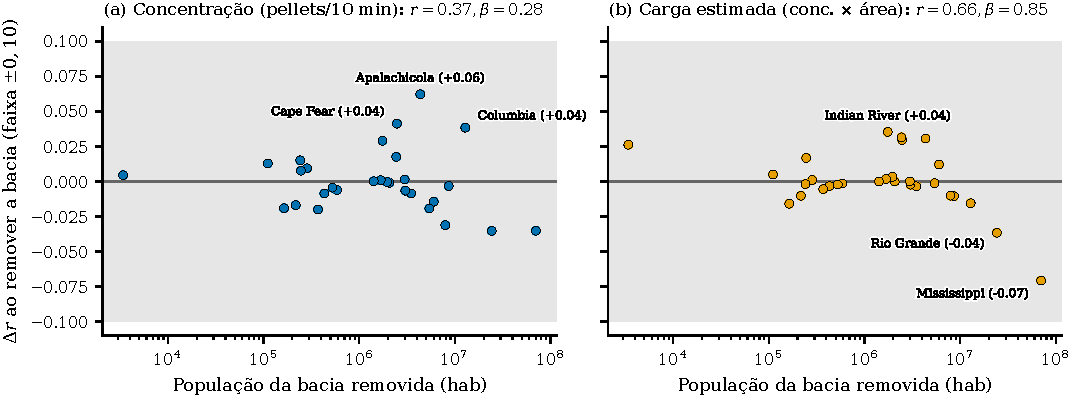
\includegraphics[width=0.6\textwidth]{leave_one_out}%
	}{%
		\Fonte{elaborado pelo autor.}%
		\Nota{A faixa cinza marca $|\Delta r| \leq 0{,}1$.}%
	}
\end{figure}

\section{Distribuições de tamanho}
\label{sec:res-distribuicoes}

A \autoref{fig:leis-potencia} e a \autoref{tab:leis-potencia} mostram os ajustes de cauda das áreas das bacias, das populações das bacias e das populações das manchas urbanas. As três distribuições têm cauda pesada, e em todas a lei de potência é fortemente preferida à exponencial.

\begin{figure}[ht!]
	\centering
	\Caption{\label{fig:leis-potencia}Distribuições complementares acumuladas das áreas e populações das bacias e das populações das manchas urbanas}
	\IBGEtab{}{%
		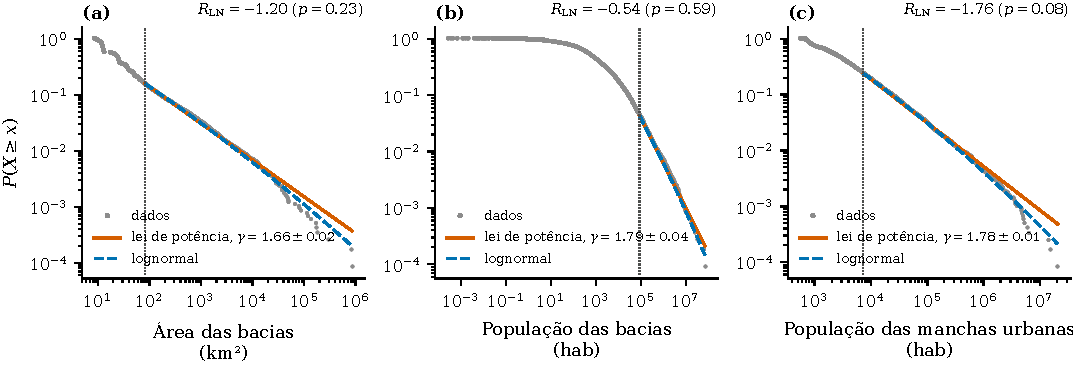
\includegraphics[width=\textwidth]{leis_potencia}%
	}{%
		\Fonte{elaborado pelo autor.}%
		\Nota{Linhas: lei de potência (contínua) e lognormal (tracejada) ajustadas acima de $x_{\min}$ (linha vertical pontilhada). $R_{\mathrm{LN}}$ é a razão de verossimilhança normalizada entre a lei de potência e a lognormal.}%
	}
\end{figure}

\begin{table}[ht!]
	\centering
	\Caption{\label{tab:leis-potencia}Ajustes de cauda pelo método CSN}
	\IBGEtab{}{%
		\small
		\begin{tabular}{lrrrrrr}
			\toprule
			\textbf{Distribuição} & \textbf{$n$} & \textbf{$x_{\min}$} & \textbf{Cauda} & \textbf{$\hat{\gamma}$} & \textbf{$R_{\mathrm{LN}}$ ($p$)} & \textbf{$R_{\mathrm{exp}}$ ($p$)} \\
			\midrule
			Área das bacias (km$^2$) & 11.794 & 82 & 1.877 & $1{,}655 \pm 0{,}015$ & $-1{,}20$ (0,23) & 8,19 ($<10^{-15}$) \\
			População das bacias & 11.134 & 86.142 & 482 & $1{,}795 \pm 0{,}036$ & $-0{,}54$ (0,59) & 5,93 ($<10^{-8}$) \\
			População das manchas & 12.185 & 7.301 & 2.939 & $1{,}782 \pm 0{,}014$ & $-1{,}76$ (0,08) & 10,99 ($<10^{-27}$) \\
			\bottomrule
		\end{tabular}%
	}{%
		\Fonte{elaborado pelo autor.}%
		\Nota{Área das bacias: apenas as que não tocam a borda. $R_{\mathrm{LN}}$ e $R_{\mathrm{exp}}$: razões de verossimilhança normalizadas entre a lei de potência e a lognormal e a exponencial; valores positivos favorecem a lei de potência.}%
	}
\end{table}

A área das bacias segue uma lei de potência com $\hat{\gamma} = 1{,}66$ a partir de 82 km$^2$, indistinguível da lognormal. O expoente é maior que os valores de 1,4 a 1,5 típicos da distribuição de áreas de sub-bacias aninhadas numa rede fluvial \cite{rodrigueziturbe1997,maritan1996}, o que é esperado: aqui as bacias não são aninhadas, mas uma partição do continente em bacias costeiras disjuntas, e as bacias grandes ``roubam'' área das vizinhas. A população das bacias tem cauda com $\hat{\gamma} = 1{,}80$, também indistinguível da lognormal. A população das manchas urbanas, com $x_{\min}$ mais baixo que no ajuste do primeiro \textit{notebook}, dá $\hat{\gamma} = 1{,}78$, ou seja, $\alpha = 1/(\hat{\gamma} - 1) \approx 1{,}28$, coerente com a concavidade discutida na \autoref{sec:res-rank-size}; nesse caso, a lognormal é marginalmente preferida ($p = 0{,}08$).

\section{Discussão}
\label{sec:discussao}

\subsection{O que os resultados dizem sobre a hipótese}

A hipótese de trabalho era que a quantidade de microplástico na foz cresce com a população da bacia. Os resultados a sustentam apenas em parte. A associação entre população e concentração de \textit{pellets} é positiva em todos os raios testados, estável entre 10 e 50 km e com IC que exclui o zero em $R_{\mathrm{maioria}}$. Mas é fraca, com a população explicando cerca de 13\% da variância, fica no limite da significância estatística e enfraquece quando as contagens zero são incluídas. O indicador de quantidade dá uma relação mais forte, mas herda a correlação entre população e área e não constitui evidência independente.

O expoente sublinear da concentração, $\beta \approx 0{,}28$, tem pelo menos quatro explicações possíveis, que não se excluem.

\begin{enumerate}
	\item \textbf{Diluição.} Bacias mais populosas tendem a ser maiores e a ter vazões maiores. Se a carga de plástico cresce com a população, mas a vazão cresce com a área, a concentração na foz cresce menos que a carga. A concentração numa praia não é uma carga, e uma relação linear entre população e carga é compatível com uma relação sublinear entre população e concentração.
	\item \textbf{Fonte industrial.} Os \textit{pellets} são um microplástico primário cuja perda está ligada à produção e ao transporte de resinas, e não ao consumo \cite{karlsson2018}. As maiores contagens estão na costa do Texas \cite{tunnell2020}, onde se concentra a indústria petroquímica, e não necessariamente nas bacias mais populosas. A população da bacia é, nesse caso, um indicador indireto da atividade industrial.
	\item \textbf{Transporte costeiro.} Uma vez no mar, os \textit{pellets} são redistribuídos por correntes e pela deriva litorânea e depositados em praias que podem estar a dezenas de quilômetros da foz de origem. O sítio mais próximo pode refletir a soma de várias fozes.
	\item \textbf{Ruído amostral.} A maioria dos sítios associados às bacias tem uma única amostra, feita num único dia, e as contagens de \textit{pellets} variam muito com o tempo, as marés e as tempestades.
\end{enumerate}

\subsection{O papel das escolhas metodológicas}

Algumas escolhas feitas ao longo do trabalho protegem os resultados de interpretações otimistas. Os parâmetros do CCA foram fixados pela lei de Zipf antes de qualquer contato com os dados de plástico, e a varredura mostrou que o critério escolhe uma região estável da matriz de parâmetros e não um ponto isolado. O raio de aceitação não foi escolhido pelo resultado, mas por um critério de cobertura dos sítios, e a varredura completa mostra que o resultado não depende criticamente dele. O $r = 0{,}94$ obtido com $R = 2$ km, que seria o resultado mais ``favorável'', foi reportado como o que é: uma flutuação de seis pontos. As contagens zero, que precisam sair do ajuste em log-log, foram analisadas à parte com uma medida de postos.

Outras escolhas limitam o alcance dos resultados:

\begin{itemize}
	\item \textbf{Resolução do relevo.} A reamostragem para 2$'$, imposta pela implementação em Python puro do IPBA, faz com que a foz seja conhecida com precisão de cerca de 3,7 km e fragmenta estuários complexos, como o de Nova York, em muitas micro-bacias. Um ``sítio a até 1 km'' significa a até 1 km desse pixel.
	\item \textbf{Bacias truncadas.} A caixa corta as cabeceiras mais ao norte das bacias do Mississippi e do São Lourenço e as bacias que drenam para a Baía de Hudson; o IPBA atribui as partes dentro da caixa às bacias vizinhas.
	\item \textbf{Cobertura das coletas.} O \textit{Nurdle Patrol} concentra-se no Golfo do México. Das 138 bacias principais, apenas 52 têm sítio a até 38 km, e o México, a América Central e o Caribe contribuem com poucas delas. As bacias com medição não são uma amostra aleatória das bacias do continente.
	\item \textbf{Tipo de microplástico.} Os \textit{pellets} são um tipo específico de microplástico primário, e os resultados não se estendem automaticamente aos microplásticos secundários, como fibras e fragmentos, que têm fontes difusas e mais diretamente ligadas ao consumo.
	\item \textbf{Concentração versus carga.} A contagem por 10 minutos de busca numa praia é uma medida de concentração local, não da carga transportada pelo rio. Um teste mais direto da hipótese exigiria medições de carga fluvial, que não estão disponíveis numa escala continental.
\end{itemize}

	\chapter{Conclusão}
\label{chap:conclusao}

Esta dissertação testou se a população que vive numa bacia hidrográfica está associada ao microplástico medido na foz dessa bacia, na América do Norte e Central, dos Estados Unidos e sul do Canadá até o Canal do Panamá. Para isso, construiu um \textit{pipeline} que cruza três bases públicas e independentes: o relevo do GEBCO 2024, a população do GPW v4 e as contagens de \textit{pellets} plásticos do \textit{Nurdle Patrol} no banco de microplásticos marinhos da NOAA.

\section{Síntese dos resultados}

\textbf{Bacias.} O IPBA, com todos os pixels de terra vizinhos ao oceano como saídas, particionou o continente em 11.851 bacias costeiras sem nenhuma lista de rios. As 138 maiores cobrem 90\% da área de terra e reproduzem as grandes bacias conhecidas, do Mississippi ao Balsas, e somam 74\% da população da região.

\textbf{Manchas urbanas.} A calibração do CCA pela lei de Zipf, feita numa grade de 15 mil combinações de parâmetros por um algoritmo de união e busca que reproduz o CCA exatamente, escolheu $D^{*} = 1.010$ hab/km$^2$ e $\ell = 1{,}7$ km. Com esses valores, as 12.185 manchas urbanas seguem a lei de Zipf no topo do \textit{ranking} ($\hat{\alpha}$ entre 0,93 e 1,08 para as 50, 100 e 200 maiores), mas a distribuição completa é côncava, com $\alpha \approx 1{,}22$ na cauda ajustada pelo método CSN. O piso físico para $\ell$ mostrou-se necessário para evitar soluções degeneradas.

\textbf{Repartição.} As 618 manchas que cruzam divisores de água somam 41\% da população urbana, e a sua repartição entre as bacias muda substancialmente a população atribuída a cada foz. O método atribuiu corretamente cidades interiores, como a Cidade do México, Guadalajara e Monterrey, a fozes distantes centenas de quilômetros, mas deixou grandes cidades litorâneas em estuários fragmentados, como Nova York, fora das bacias principais.

\textbf{Microplástico e população.} Com o raio de aceitação que contém a maioria dos sítios de coleta ($R = 38$ km), 52 bacias têm medição, 29 com contagem positiva. Nessas 29, a concentração de \textit{pellets} cresce de forma sublinear com a população, com $\beta = 0{,}28$ (IC de 95\%: 0,11 a 0,54) e $r = 0{,}37$. A relação é estável entre 10 e 50 km, não depende de nenhuma bacia isolada, mas é fraca: a população explica cerca de 13\% da variância, e a correlação de postos cai para $\rho_s = 0{,}25$ ($p = 0{,}07$) quando as contagens zero são incluídas. O indicador de quantidade (concentração $\times$ área) dá $\beta = 0{,}85$ e $r = 0{,}66$, mas dois terços desse expoente vêm da correlação entre população e área das bacias. Com medição garantida, a até 1 km da foz, só três bacias estão disponíveis.

\section{Resposta à pergunta de pesquisa}

Os dados públicos disponíveis sustentam, no máximo, uma associação \textbf{positiva, sublinear e fraca} entre a população de uma bacia e a concentração de \textit{pellets} plásticos na sua foz. Eles não permitem afirmar que a população determina o microplástico que chega ao mar, nem estimar com precisão o expoente dessa relação. A principal limitação não está nos métodos, mas nos dados de plástico: as coletas se concentram no Golfo do México, raramente coincidem com fozes, têm em geral uma única amostra por sítio e medem um tipo de microplástico, os \textit{pellets}, cuja fonte é mais industrial do que populacional.

Esse resultado é, em si, relevante. Os modelos globais de emissão de plástico por rios usam a população da bacia como variável explicativa central \cite{lebreton2017,meijer2021}. A fraqueza da associação encontrada aqui com medições de campo independentes sugere cautela na extrapolação desses modelos e reforça a necessidade de medições sistemáticas nas fozes.

\section{Contribuições}

As contribuições do trabalho são:

\begin{itemize}
	\item um \textit{pipeline} reprodutível e aberto que integra relevo, população e microplástico numa análise por bacia, executável a partir de dois \textit{notebooks};
	\item o uso do IPBA com todos os \textit{sinks} costeiros e de um critério de cobertura de área para selecionar as bacias principais sem listas manuais nem limiares de área;
	\item um algoritmo de varredura do CCA em tempo quase linear por valor de $\ell$, exato em relação ao CCA, que torna viável explorar milhares de combinações de parâmetros sobre grades de dezenas de milhões de células;
	\item um critério de calibração do CCA pela lei de Zipf robusto a variações do tamanho da amostra e com um piso físico para a distância de ligação;
	\item a repartição das manchas urbanas entre bacias e a demonstração de que ela afeta quase metade da população urbana;
	\item uma análise explícita da sensibilidade ao raio de aceitação, que evita escolher o raio pelo resultado.
\end{itemize}

\section{Trabalhos futuros}

Os resultados sugerem as seguintes extensões.

\begin{itemize}
	\item \textbf{Agrupar \textit{sinks} de estuários.} Unir os \textit{sinks} de uma mesma baía ou estuário antes do IPBA, por exemplo agrupando pixels de costa separados por menos de alguns quilômetros de água, permitiria associar cidades como Nova York a uma única foz.
	\item \textbf{Relevo em resolução maior.} Uma implementação compilada do IPBA, com rótulos de 32 bits, permitiria usar o GEBCO na resolução nativa de 15$''$, localizando as fozes com precisão de algumas centenas de metros e aumentando o número de bacias com medição garantida.
	\item \textbf{Outras medidas de plástico.} Aplicar o mesmo \textit{pipeline} a medições de microplástico secundário na água ou no sedimento de estuários, ou a medições de carga fluvial, que testariam a hipótese de forma mais direta.
	\item \textbf{Modelos para as contagens.} Tratar as contagens zero com modelos de contagem, como regressões binomiais negativas com inflação de zeros, em vez de excluí-las do ajuste em log-log.
	\item \textbf{Covariáveis industriais.} Incluir a localização de fábricas de resina e terminais portuários como covariável, para separar o efeito da população do efeito da indústria no caso dos \textit{pellets}.
	\item \textbf{Transporte costeiro.} Ponderar os sítios por um modelo simples de deriva litorânea, em vez de usar apenas o sítio mais próximo da foz.
	\item \textbf{Outras regiões.} Aplicar o \textit{pipeline} a outras regiões com boa cobertura de coletas, como a Europa ou o litoral brasileiro, onde há programas de monitoramento de \textit{pellets} em praias.
\end{itemize}


	% Elementos pós-textuais
	\bibliography{elementos-pos-textuais/referencias}
	\imprimirglossario
	\imprimirapendices
		\chapter{Reprodutibilidade}
\label{apendice:reprodutibilidade}

Todo o processamento desta dissertação está em dois \textit{notebooks} Jupyter, desenvolvidos para o Google Colab, que baixam os dados e o código de terceiros em tempo de execução. Este apêndice lista os arquivos, os parâmetros e as saídas de cada etapa.

\section{Ordem de execução}

\begin{enumerate}
	\item \texttt{01\_Zipf\_calibracao\_CCA.ipynb}: lê o GPW v4, executa a varredura de $(D^{*}, \ell)$, escolhe o par pelo critério $\Delta$, verifica o resultado com o \texttt{cca\_grid}, ajusta a distribuição das manchas pelo método CSN e grava \texttt{results/cca\_calibracao.json}.
	\item \texttt{02\_Micro\_Plastic.ipynb}: lê os parâmetros do CCA do arquivo anterior e executa o recorte, o IPBA, a seleção das bacias principais, o CCA, a repartição das manchas, a associação do microplástico às fozes, a varredura do raio e os ajustes de escala. O IPBA, em Python puro, é a etapa mais lenta.
\end{enumerate}

\section{Dados e código de terceiros}

\begin{itemize}
	\item GEBCO 2024: lido diretamente da cópia em formato COG em \url{https://data.source.coop/alexgleith/gebco-2024/GEBCO_2024.tif} \cite{gebco2024}.
	\item GPW v4.11, contagem de população de 2020, 30 segundos de arco \cite{gpw4}.
	\item Banco de microplásticos marinhos do NCEI/NOAA, exportado em CSV \cite{nyadjro2023}.
	\item IPBA: \url{https://github.com/erneson/IPBA} \cite{ipba}.
	\item Pacote CCA com a função \texttt{cca\_grid}: \url{https://github.com/skaduhs5232/CCA}.
\end{itemize}

\section{Parâmetros}

A \autoref{tab:parametros} lista todos os parâmetros do \textit{pipeline} e a origem de cada valor. Nenhum deles foi ajustado a partir da relação entre população e microplástico.

\begin{table}[ht!]
	\centering
	\Caption{\label{tab:parametros}Parâmetros do \textit{pipeline}}
	\IBGEtab{}{%
		\small
		\begin{tabular}{p{4.6cm}p{3.0cm}p{6.4cm}}
			\toprule
			\textbf{Parâmetro} & \textbf{Valor} & \textbf{Origem} \\
			\midrule
			Caixa de estudo & $[-125, -65] \times [7, 50]$ & Região com maior cobertura do \textit{Nurdle Patrol}; inclui a bacia do Mississippi inteira \\
			Corte do Canal do Panamá & lon $> -79^\circ$ e lat $< 12{,}6^\circ$ & Exclui a América do Sul sem partir a Cidade do Panamá \\
			Reamostragem do GEBCO & $8 \times 8$ (2$'$) & Limite de 65.535 \textit{sinks} do IPBA \\
			Vizinhança dos \textit{sinks} e do IPBA & 4 células & Padrão do IPBA \\
			Cobertura das bacias principais $P$ & 0,90 & Especificação do trabalho \\
			Grade de $D^{*}$ & 10 a 3.000 hab/km$^2$, passo 10 & Especificação do trabalho \\
			Grade de $\ell$ & 100 a 5.000 m, passo 100 & Especificação do trabalho \\
			$\ell_{\min}$ & 1.400 m & Diagonal entre células do GPW (1.307 m) \\
			$N$ do estimador de Hill & 50, 100 e 200 & Topo do \textit{ranking} \\
			$D^{*}$ escolhido & 1.010 hab/km$^2$ & Mínimo de $\Delta$ (\autoref{eq:delta}) \\
			$\ell$ escolhido & 1.700 m & Mínimo de $\Delta$ (\autoref{eq:delta}) \\
			Realocação costeira & até 8 células do GPW ($\approx 7$ km) & Diferença de resolução entre GEBCO reamostrado e GPW \\
			Margem da busca de sítios & 50 km & Maior raio testado \\
			Raio de aceitação $R$ & 1 a 50 km, passo 1 & Especificação do trabalho \\
			$R_{\mathrm{maioria}}$ & 38 km & Menor $R$ com $\geq 50\%$ dos sítios \\
			Reamostragens do \textit{bootstrap} & 10.000 (2.000 na varredura de $R$) & Convenção \\
			Permutações & 10.000 (2.000 na varredura de $R$) & Convenção \\
			Reamostragens do teste CSN & 200 & Convenção \\
			\bottomrule
		\end{tabular}%
	}{%
		\Fonte{elaborado pelo autor.}%
	}
\end{table}

\section{Saídas}

As saídas são gravadas na pasta \texttt{results/} com o sufixo \texttt{na\_panama}:

\begin{itemize}
	\item \texttt{cca\_calibracao.json}: parâmetros escolhidos, expoentes de Hill, $\Delta$, critério e ajuste CSN;
	\item \texttt{zipf\_matriz\_*.npz} e \texttt{zipf\_curva\_alpha1\_*.csv}: matriz de expoentes e curva $\alpha = 1$;
	\item \texttt{zipf\_clusters\_*.csv}: todas as manchas urbanas com população, área, centroide e nome;
	\item \texttt{bacias\_*.csv}: bacias principais com área, população, população urbana, foz, sítio mais próximo, distância e microplástico;
	\item \texttt{manchas\_por\_bacia\_*.csv}: pedaços das manchas em cada bacia;
	\item \texttt{varredura\_raio\_*.csv} e \texttt{escala\_pop\_lixo\_*.csv}: varredura do raio e ajustes de escala;
	\item \texttt{leis\_potencia\_*.csv}: ajustes de cauda;
	\item figuras em PDF e PNG, as mesmas usadas nesta dissertação.
\end{itemize}

		\chapter{Bacias principais com sítio de coleta a até 38 km da foz}
\label{apendice:bacias}

A \autoref{tab:apendice-bacias} lista as 52 bacias principais com sítio do \textit{Nurdle Patrol} a até $R_{\mathrm{maioria}} = 38$ km da foz, ordenadas pela população. As 29 bacias com contagem positiva entram nos ajustes em log-log da \autoref{sec:res-alometria}; as 23 com contagem zero entram apenas nas correlações de postos. ``Bacia'' é o rótulo do \textit{sink} da foz no IPBA; ``Lon.'' e ``Lat.'' são as coordenadas do pixel da foz; ``Dist.'' é a distância da foz ao sítio mais próximo.

{\small
\begin{longtable}{rrrrrrrc}
	\caption{\label{tab:apendice-bacias}Bacias principais com sítio a até 38 km da foz} \\
	\toprule
	\textbf{Bacia} & \textbf{Lon.} & \textbf{Lat.} & \textbf{Área (km$^2$)} & \textbf{Pop. (mi)} & \textbf{Dist. (km)} & \textbf{\textit{Pellets}/10 min} & \textbf{No ajuste} \\
	\midrule
	\endfirsthead
	\toprule
	\textbf{Bacia} & \textbf{Lon.} & \textbf{Lat.} & \textbf{Área (km$^2$)} & \textbf{Pop. (mi)} & \textbf{Dist. (km)} & \textbf{\textit{Pellets}/10 min} & \textbf{No ajuste} \\
	\midrule
	\endhead
	\bottomrule
	\multicolumn{8}{l}{\footnotesize $^{*}$ Bacia truncada pela borda da caixa. Fonte: elaborado pelo autor.} \\
	\endlastfoot
		4479$^{*}$ & $-91{,}18$ & $29{,}58$ & 3.150.557 & 70,20 & 37,8 & 47,0 & sim \\
		5937 & $-97{,}32$ & $26{,}28$ & 849.584 & 24,24 & 9,7 & 57,0 & sim \\
		1136$^{*}$ & $-123{,}58$ & $46{,}22$ & 1.012.275 & 12,86 & 35,7 & 5,0 & sim \\
		2591 & $-122{,}25$ & $38{,}08$ & 177.542 & 9,85 & 21,3 & 0,0 & não \\
		3868 & $-87{,}98$ & $30{,}72$ & 171.579 & 8,62 & 2,0 & 19,0 & sim \\
		4263 & $-94{,}78$ & $29{,}78$ & 46.863 & 8,33 & 3,3 & 0,0 & não \\
		2228 & $-75{,}52$ & $39{,}65$ & 26.636 & 7,94 & 4,2 & 123,0 & sim \\
		2492 & $-77{,}02$ & $38{,}35$ & 35.859 & 7,43 & 35,9 & 0,0 & não \\
		3395 & $-118{,}08$ & $33{,}75$ & 5.988 & 6,00 & 0,0 & 41,0 & sim \\
		4372 & $-94{,}98$ & $29{,}68$ & 10.417 & 5,41 & 0,0 & 81,0 & sim \\
		6314 & $-81{,}05$ & $25{,}15$ & 31.631 & 4,85 & 4,3 & 0,0 & não \\
		3483 & $-79{,}35$ & $33{,}18$ & 40.876 & 4,70 & 36,4 & 0,0 & não \\
		4146 & $-85{,}58$ & $30{,}05$ & 49.156 & 4,35 & 15,9 & 1,0 & sim \\
		4863 & $-95{,}22$ & $29{,}05$ & 80.218 & 3,48 & 1,4 & 42,0 & sim \\
		5124 & $-96{,}45$ & $28{,}32$ & 28.097 & 3,03 & 1,1 & 38,0 & sim \\
		9208 & $-95{,}85$ & $18{,}82$ & 43.985 & 2,99 & 4,0 & 12,0 & sim \\
		3386 & $-79{,}25$ & $33{,}78$ & 36.791 & 2,81 & 32,5 & 0,0 & não \\
		1912 & $-72{,}92$ & $41{,}28$ & 30.953 & 2,75 & 15,0 & 0,0 & não \\
		3284 & $-77{,}88$ & $34{,}08$ & 23.128 & 2,48 & 3,7 & 1,0 & sim \\
		4980 & $-95{,}78$ & $28{,}75$ & 110.090 & 2,44 & 5,5 & 471,0 & sim \\
		3970 & $-81{,}42$ & $30{,}42$ & 13.689 & 2,39 & 13,3 & 0,0 & não \\
		4095 & $-89{,}62$ & $30{,}18$ & 27.922 & 2,07 & 17,5 & 16,0 & sim \\
		936 & $-122{,}35$ & $47{,}62$ & 5.103 & 2,05 & 6,8 & 0,0 & não \\
		3126 & $-76{,}95$ & $35{,}05$ & 12.760 & 1,97 & 3,8 & 14,3 & sim \\
		5126 & $-80{,}65$ & $28{,}32$ & 9.561 & 1,75 & 2,5 & 1,0 & sim \\
		3480 & $-117{,}38$ & $33{,}22$ & 5.139 & 1,68 & 9,6 & 39,0 & sim \\
		3612 & $-80{,}92$ & $32{,}08$ & 36.271 & 1,63 & 11,7 & 0,0 & não \\
		4269 & $-93{,}55$ & $29{,}78$ & 47.887 & 1,42 & 2,1 & 10,0 & sim \\
		8138 & $-89{,}65$ & $21{,}25$ & 12.279 & 1,37 & 2,5 & 0,0 & não \\
		8390 & $-105{,}25$ & $20{,}68$ & 15.622 & 1,10 & 7,0 & 0,0 & não \\
		4809 & $-82{,}82$ & $29{,}15$ & 28.166 & 0,91 & 19,0 & 0,0 & não \\
		1002 & $-122{,}55$ & $47{,}28$ & 7.779 & 0,89 & 27,3 & 0,0 & não \\
		1954 & $-73{,}08$ & $41{,}18$ & 5.099 & 0,79 & 0,0 & 0,0 & não \\
		8260 & $-97{,}35$ & $20{,}98$ & 6.129 & 0,58 & 25,4 & 5,0 & sim \\
		2579 & $-122{,}52$ & $38{,}12$ & 4.947 & 0,53 & 29,8 & 0,0 & não \\
		3986 & $-88{,}58$ & $30{,}38$ & 20.996 & 0,53 & 2,5 & 7,0 & sim \\
		800 & $-122{,}22$ & $48{,}02$ & 7.574 & 0,48 & 14,8 & 0,0 & não \\
		1559 & $-124{,}18$ & $43{,}72$ & 23.920 & 0,43 & 28,1 & 5,0 & sim \\
		418$^{*}$ & $-122{,}58$ & $48{,}78$ & 13.387 & 0,42 & 2,5 & 0,0 & não \\
		2875 & $-121{,}75$ & $36{,}75$ & 12.945 & 0,37 & 3,0 & 1,0 & sim \\
		3530 & $-79{,}95$ & $32{,}78$ & 8.207 & 0,36 & 0,0 & 0,0 & não \\
		3969 & $-86{,}22$ & $30{,}42$ & 12.178 & 0,28 & 5,5 & 16,0 & sim \\
		5307 & $-97{,}52$ & $27{,}85$ & 44.239 & 0,25 & 1,2 & 14,0 & sim \\
		4272 & $-93{,}45$ & $29{,}78$ & 6.965 & 0,24 & 4,3 & 19,0 & sim \\
		3906 & $-87{,}12$ & $30{,}52$ & 11.079 & 0,22 & 3,4 & 4,0 & sim \\
		7968 & $-87{,}95$ & $21{,}55$ & 7.047 & 0,20 & 5,4 & 0,0 & não \\
		5604 & $-82{,}12$ & $26{,}95$ & 5.004 & 0,19 & 22,6 & 0,0 & não \\
		3907 & $-87{,}02$ & $30{,}52$ & 5.612 & 0,16 & 13,0 & 4,0 & sim \\
		645 & $-122{,}38$ & $48{,}25$ & 8.574 & 0,12 & 10,7 & 0,0 & não \\
		5539 & $-97{,}38$ & $27{,}18$ & 11.505 & 0,11 & 0,0 & 13,0 & sim \\
		5181 & $-97{,}05$ & $28{,}12$ & 5.807 & 0,06 & 0,8 & 0,0 & não \\
		5636 & $-97{,}48$ & $26{,}85$ & 5.556 & 0,00 & 10,4 & 5,0 & sim \\
\end{longtable}
}


\end{document}
